
\chapter{A teljes indukció (különböző változatai, a végtelen leszállás elve)}\label{chap:indukcio}
\begin{description}
{\large \item [{Szerző:}] Boga Zsombor (Didaktikai mesteri -- Matematika, I. év)}
\end{description}
A matematikai indukció a matematikában használt egyik legfontosabb
bizonyítási (és nemcsak bizonyítási, hanem például definiálási) módszer
is. A matematikai indukciót mint bizonyítási módszert először Pascal
írta le a kombinatorikai összefüggések bizonyításakor a következőképpen: 
\begin{quote}
„Bár ez az állítás végtelen sok esetet tartalmaz, igen rövid bizonyítást
adok rá, amely két lemmán alapszik. Az első azt állítja, hogy a kijelentés
igaz az első sorra. A második pedig azt mondja ki: ha a kijelentés
igaz egy adott sorra, akkor szükségszerűen igaz a következő sorra
is.” 
\end{quote}
Ebben a fejezetben a \emph{teljes indukció}, annak különböző változatai,
valamint a \emph{végtelen leszállás} módszere kerül bemutatásra (\ref{formai}).
Ezt követően a módszerek \emph{precíz algebrai} levezetését és helyességének
bizonyítását tárgyaljuk (\ref{algebrai}).

\section*{Az indukció különböző formái}

\label{formai}

%Ez az alfejezet összefoglalja a matematikai teljes indukció módszerét
%és annak ekvivalens formáit.

\subsection*{A matematikai indukció elve }
\begin{theorem}{thm:indukcio-elv} Rendeljünk hozzá minden $n\in\mathbb{N}$
természetes számhoz egy $P(n)$ kijelentést. Ha teljesülnek a következő
feltételek: 
\begin{enumerate}
\item $P(0)$ igaz, 
\item bármely $n\in\mathbb{N}$ esetén, ha $P(n)$ igaz, akkor $P(n+1)$
is igaz, 
\end{enumerate}
akkor $P(n)$ igaz minden $n\in\mathbb{N}$ esetén. 
\end{theorem}


\subsection*{A matematikai indukció variánsai}
\begin{theorem}[Első variáns]{thm:indukcio-varians1} Legyen $a\in\mathbb{N}$ egy természetes
szám. Minden $n\ge a$ számhoz hozzárendelünk egy $P(n)$ kijelentést.
Ha teljesülnek a következő feltételek: 
\begin{enumerate}
\item $P(a)$ igaz, 
\item $\forall k\in\mathbb{N},\,k\ge a$ esetén, ha $P(k)$ igaz, akkor
$P(k+1)$ is igaz, 
\end{enumerate}
akkor $P(n)$ igaz $\forall n\ge a$ esetén. 
\end{theorem}

\begin{theorem}[Második variáns]{thm:indukcio-varians2} Ha $a\in\mathbb{N}$
és minden $n\ge a$ számhoz hozzárendelünk egy $P(n)$ kijelentést,
amely teljesíti a következő feltételeket: 
\begin{enumerate}
\item $P(a),\,P(a+1),\,P(a+2),\ldots,P(a+k-1)$ igazak \quad{}($k$ egy
rögzített szám), 
\item Bármely $n\ge a$ esetén, ha $P(n)$ igaz, akkor $P(n+k)$ is igaz, 
\end{enumerate}
akkor $P(n)$ igaz $\forall n\ge a$ esetén. 
\end{theorem}

\begin{theorem}[Harmadik variáns]{thm:indukcio-varians3} Legyen $a\in\mathbb{N}$
egy rögzített természetes szám. Ha minden $n\ge a$ számhoz hozzárendelünk
egy $P(n)$ kijelentést, amely teljesíti a következő feltételeket: 
\begin{enumerate}
\item $P(a)$ igaz, 
\item $\forall n\in\mathbb{N}$ esetén, ha $P(k)$ igaz minden $n\ge k\ge a$-ra,
akkor $P(n+1)$ is igaz, 
\end{enumerate}
akkor $P(n)$ igaz $\forall n\ge a$ esetén. 
\end{theorem}

\begin{theorem}[Negyedik variáns]{thm:indukcio-varians4} Legyen $a\in\mathbb{N}$
egy rögzített természetes szám. Minden $n\ge a$ számhoz hozzárendelünk
egy $P(n)$ kijelentést, amely teljesíti a következő feltételeket
(legyen $k$ szintén egy rögzített természetes szám): 
\begin{enumerate}
\item $P(a),\,P(a+1),\,P(a+2),\ldots,P(a+k-1)$ igazak, 
\item Ha bármely $m\in\mathbb{N},\,n\le m\le n+k-1$ esetén $P(m)$ igaz,
akkor $P(n+k)$ is igaz, 
\end{enumerate}
akkor $P(n)$ igaz minden $n\in\mathbb{N},\,n\ge a$ esetén. 
\end{theorem}


\subsection*{Indukció a valós számok halmazán}

Az eddig bemutatott indukciós bizonyítási variánsok közös vonása,
hogy természetes számokra vonatkozó kijelentések igazolására szolgálnak.
A matematikai indukció módszerével azonban olyan állításokat is bizonyíthatunk,
amelyek nem természetes, hanem pozitív valós számokra vonatkoznak.
\begin{theorem}[Indukció a valós számok halmazán]{thm:valos-szamok-indukcio} Tegyük fel, hogy
$x\in\mathbb{R}^{+}$ esetén adott egy $P(x)$ kijelentés, és teljesülnek
az alábbi feltételek: 
\begin{enumerate}
\item $P(x)$ igaz minden $x\in[0,1]$ esetén, 
\item Bármely $x\ge0$ esetén, ha $P(x)$ igaz, akkor $P(x+1)$ is igaz, 
\end{enumerate}
akkor $P(x)$ igaz minden $x\ge0$ valós számra. 
\end{theorem}


\subsection*{Többváltozós indukció}
\begin{theorem}[Többváltozós indukció elve]{thm:tobbvaltozos-indukcio} Tegyük fel, hogy
$n_{0},m_{0}\in\mathbb{N}$, és $P(n,m)$ egy $n$-től és $m$-től
függő predikátum. Ha teljesülnek az alábbi feltételek: 
\begin{enumerate}
\item $P(n_{0},m_{0})$ igaz, 
\item Ha $P(n',m')$ igaz bármely olyan $n',m'$-re, amelyekre $n'+m'<n+m$,
akkor $P(n,m)$ is igaz, 
\end{enumerate}
akkor $P(n,m)$ igaz bármely $n,m\in\mathbb{N},\,n\ge n_{0},\,m\ge m_{0}$
esetén. 
\end{theorem}


\subsection*{A végtelen leszállás elve}

A végtelen leszállás a teljes indukció indirekt változata, amelyben
nem azt bizonyítjuk be, hogy ha egy természetes számokra vonatkozó
állítás igaz az összes $n$-nél kisebb számra, akkor igaz $n$-re
is, hanem azt, hogy ha az $n$-re nem teljesül az állítás, akkor van
egy $n$-nél kisebb pozitív egész is, amire nem teljesül. Egy lehetséges
megfogalmazás a következő:
\begin{theorem}[A végtelen leszállás elve]{thm:vegtelen-leszallas} Legyen $P(n)$ egy, a természetes
számokra vonatkozó kijelentés. Tegyük fel, hogy van olyan $n_{0}\in\mathbb{N}$,
melyre $P(n_{0})$ nem igaz. Legyen 
\[
H\;=\;\{\,n\in\mathbb{N}\;\mid\;P(n)\text{ nem igaz}\}.
\]
Továbbá tegyük fel, hogy $H$-nak van legkisebb eleme. Ha azonban
bármely $n\in\mathbb{N}$ esetén mindig találunk $m\in H$ olyat,
hogy $m<n$, akkor $H$-nak nem lehetne minimális eleme, ami ellentmondás.
Így a feltételezés hibás, és minden $n$-re igaz $P(n)$. 
\end{theorem}

Ezzel ellentmondásra jutunk, hiszen feltettük, hogy $n_{0}$ is hibás.
Így belátjuk, hogy $H$-nak nem lehet minimuma, vagyis a kezdeti feltevés
hibás, és mégis igaznak bizonyul a $P(n)$ minden $n$-re.

\section*{Az indukció algebrai megalapozása rendezési relációkkal}

\label{algebrai}

\subsection*{Rendezési relációk}
\begin{theorem}{thm:rendezesi-relacio} Legyen $\rho=(A,A,R)$ egy homogén
reláció. Ha $\rho$ \emph{reflexív}, \emph{tranzitív} és \emph{antiszimmetrikus},
akkor $\rho$ \emph{rendezési reláció}, és $(A,\rho)$ egy \emph{rendezett
halmaz}. 
\end{theorem}

\begin{definition}{def:teljesen_rendezett_halmaz}
Azt mondjuk, hogy $(A,\rho)$ \emph{teljesen rendezett halmaz} vagy
\emph{lánc}, ha a következő tulajdonság is teljesül: 
\[
\text{minden }x,y\in A\text{ esetén }x\rho y\text{ vagy }y\rho x,
\]
azaz $A$ bármely két eleme összehasonlítható a $\rho$ reláció szerint. 
\end{definition}

\begin{example}
1) $(\mathbb{N},\leq),(\mathbb{Z},\leq),(\mathbb{Q},\leq),(\mathbb{R},\leq)$
teljesen rendezett halmazok.\\
 2) $(\mathbb{N},\mid)$, ahol ,,\,$\mid$\," az oszthatósági reláció,
rendezett halmaz és nem teljesen rendezett, mert pl.\ 2 és 3 nem
hasonlíthatók össze, egyik sem osztója a másiknak.\\
 3) Ha $A$ egy tetszőleges halmaz, akkor $(\mathcal{P}(A),\subseteq)$
rendezett halmaz. Ha $A$-nak egynél több eleme van, akkor $(\mathcal{P}(A),\subseteq)$
nem teljesen rendezett.\\
 4) Ha $(A,\rho)$ rendezett (teljesen rendezett) halmaz és $B\subseteq A$,
akkor $(B,\rho\cap(B\times B))$ is rendezett (teljesen rendezett). 
\end{example}

\smallskip{}

Ha $\rho$ \emph{rendezési reláció}, akkor $x\rho y$ helyett gyakran
$x\leq y$-t írunk, akkor is, ha $\rho$ nem a szokásos „kisebb vagy
egyenlő" reláció. További jelölések: $x<y$, ha $x\leq y$ és $x\neq y$
(\emph{szigorú egyenlőtlenség}); $x>y$, ha $y<x$.

\medskip{}

A véges rendezett halmazokat \emph{Hasse-féle diagramokkal} ábrázoljuk.
Ha $x<y$ és ha nem létezik $z\in A$ úgy, hogy $x<z<y$, akkor az
$y$ pontot az $x$ pontnál magasabb szinten helyezzük el és a két
pontot egy egyenes szakasszal összekötjük.
\begin{example}
Legyen $A=\{x,y,z,t\}$ és tekintsük azt a rendezési relációt $A$-n,
melynek grafikonja 
\[
R=\{(x,x),(y,y),(z,z),(t,t),(x,y),(x,z),(x,t),(y,t),(z,t)\}.
\]
Ennek Hasse-diagramja a következő \emph{gyémánt} alakú ábra, ahol
az \texttt{x-y}, \texttt{x-z}, \texttt{y-t}, \texttt{z-t} élek jelzik
az „azonnali” (köztes elem nélküli) lefedést:\par \[
\begin{tikzpicture}[scale=1,>=latex,node distance=1.5cm]
  \node (x) at (0,0) {x};
  \node (y) at (-1,1.5) {y};
  \node (z) at (1,1.5) {z};
  \node (t) at (0,3) {t};

  \draw (x) -- (y);
  \draw (x) -- (z);
  \draw (y) -- (t);
  \draw (z) -- (t);
\end{tikzpicture}
\]
\par Ha a grafikon 
\[
R=\{(x,x),(y,y),(z,z),(t,t),(x,y),(x,z),(x,t),(y,z),(y,t),(z,t)\},
\]
akkor $(A,\leq)$ \emph{lánc}, és a Hasse-diagram egy \emph{függőleges
oszlop}:\par \[
\begin{tikzpicture}[scale=1,>=latex,node distance=1.2cm]
  \node (x) at (0,0)   {x};
  \node (y) at (0,1.3) {y};
  \node (z) at (0,2.6) {z};
  \node (t) at (0,3.9) {t};

  \draw (x) -- (y);
  \draw (y) -- (z);
  \draw (z) -- (t);
\end{tikzpicture}
\]\par A harmadik diagram azt a rendezési relációt adja meg, melyre
$x<y$, $x<z$, $y$ és $z$ nem hasonlítható össze, továbbá $t$
sem hasonlítható össze az $x$, $y$, $z$ egyikével sem. Ennek megfelelően
semmilyen él nem megy $t$-ből vagy $t$-be, illetve $y$ és $z$
között sincs él:\par \[
\begin{tikzpicture}[scale=1,>=latex,node distance=1.2cm]
  \node (x) at (0,0)   {x};
  \node (y) at (-1.5,1.5) {y};
  \node (z) at (1.5,1.5)  {z};
  \node (t) at (2.5,0)   {t};

  % x < y, x < z:
  \draw (x) -- (y);
  \draw (x) -- (z);

  % y, z nem összehasonlítható, és t nem viszonyul x, y, z-hez, így nincs több él.
\end{tikzpicture}
\]
\end{example}

\begin{definition}{def:rendezett_halmaz}
Legyen $(A,\leq)$ egy \emph{rendezett halmaz} és $x\in A$. Azt mondjuk,
hogy $x$ az $A$-nak \emph{legkisebb eleme} vagy \emph{minimuma}
(\emph{legnagyobb eleme} vagy \emph{maximuma}), ha 
\[
\text{minden }a\in A\text{ esetén }x\leq a\quad(\text{illetve minden }a\in A\text{ esetén }a\leq x).
\]
Jelölés: $x=\min A$ (illetve $x=\max A$). 
\end{definition}

\noindent Megjegyezzük, hogy ha létezik legkisebb elem (legnagyobb
elem), akkor csak egy ilyen van.
\begin{example}
1) $(\mathbb{N},\leq)$-ben $x=0$ legkisebb elem, legnagyobb elem
nem létezik.\\
 2) $(\mathbb{N},\mid)$-ban az 1 a legkisebb elem és a 0 a legnagyobb
elem.\\
 3) $(\mathbb{N}\backslash\{0,1\},\mid)$-ban nem létezik legkisebb
elem és nem létezik legnagyobb elem.\\
 4) $(\mathcal{P}(A),\subseteq)$-ban $\min\mathcal{P}(A)=\emptyset$
és $\max\mathcal{P}(A)=A$. 
\end{example}

\begin{definition}{def:minimalis_elem}
Az $(A,\leq)$ egy rendezett halmaznak $x\in A$ akkor \emph{minimális
eleme} (illetve \emph{maximális eleme}), ha 
\[
\forall a\in A:a\leq x\;\Rightarrow\;a=x\quad(\text{illetve }\forall a\in A:x\leq a\;\Rightarrow\;a=x).
\]
Másképp fogalmazva: $x\in A$ minimális elem, ha $A$-ban nincs olyan
$a$ elem, melyre $a<x$ (maximális elem esetén nincs $a>x$). 
\end{definition}

\begin{example}
1) $(\mathbb{N},\leq)$-ben $x=0$ minimális elem, maximális elem
nem létezik.\\
 2) $(\mathbb{N},\mid)$-ban az 1 minimális elem és 0 maximális elem.\\
 3) $(\mathbb{N}\backslash\{0,1\},\mid)$-ban a prímszámok minimális
elemek, maximális elem nem létezik. 
\end{example}

\medskip{}

Az értelmezések alapján azonnali, hogy ha létezik legkisebb (legnagyobb)
elem, akkor ez az egyetlen minimális (maximális) elem. A fordított
állítás nem igaz, például ha $A=\{2^{k}\mid k\in\mathbb{N}\}\cup\{3,9\}$,
akkor az $(A,\mid)$ rendezett halmazban a 9 az egyetlen maximális
elem és nem létezik legnagyobb elem.

Ha $(A,\leq)$ rendezett halmaz és $B\subseteq A,B\neq\emptyset$,
akkor beszélhetünk a $B$ legkisebb (legnagyobb) eleméről valmint
a $B$ minimális (maximális) elemeiről.

Ha $(A,\leq)$ teljesen rendezett halmaz, akkor a minimális elem (maximális
elem) fogalma egyenértékű a legkisebb elem (illetve legnagyobb elem)
fogalmával.

\subsection*{Jólrendezett halmazok}
\begin{definition}{def:jolrendezett_halmaz}
Legyen $(A,\leq)$ egy rendezett halmaz. Azt mondjuk, hogy $A$ \emph{jólrendezett
halmaz}, ha $A$ minden \emph{nem üres} részhalmazának létezik \emph{legkisebb
eleme}. 
\end{definition}

\begin{rem}
a) $(\mathbb{N},\leq)$ \emph{jólrendezett} halmaz.\\
 b) Ha $(A,\leq)$ jólrendezett, akkor $(A,\leq)$ \emph{teljesen
rendezett}. Fordítva nem igaz.\\
 c) Minden véges teljesen rendezett halmaz jólrendezett. 
\end{rem}

A következő tétel megmutatja, hogy \emph{jólrendezett halmazok} esetén
alkalmazható a \emph{matematikai indukció} módszere.
\begin{theorem}{thm:jolrendezett} (\emph{Jólrendezett halmazok jellemzése})
Legyen $(A,\leq)$ egy nem üres rendezett halmaz. Ekvivalensek a következő
állítások: 
\begin{itemize}
\item[(i)] $(A,\leq)$ \emph{jólrendezett}, 
\item[(ii)] $A$ \emph{teljesen rendezett}, létezik $a_{0}=\min A$, és minden
$B\subseteq A$ esetén, ha $B$ rendelkezik a következő tulajdonságokkal: 
\begin{enumerate}
\item $a_{0}\in B$, 
\item minden $a\in A$ esetén, ha $\{x\in A\mid x<a\}\subseteq B$, akkor
$a\in B$, 
\end{enumerate}
akkor $B=A$. 

\end{itemize}
\end{theorem}
\begin{proof}
(i) $\Rightarrow$ (ii) Fogadjuk el, hogy
$(A,\leq)$ jólrendezett. Akkor $A$ teljesen rendezett, és létezik
$a_{0}=\min A$. Tegyük fel, hogy (ii) második része nem igaz, azaz
létezik olyan $B\subseteq A$, melyre teljesül a) és b) és $B\neq A$.

Így $A\backslash B\neq\emptyset$ és a feltétel szerint létezik $x=\min(A\backslash B)$.
Itt $x\in A\backslash B$, azaz $x\notin B$. Továbbá $\forall y\in A:y<x\Rightarrow y\in B$
(mert ha $y\in A\backslash B$, akkor ez ellentmond $x$ definíiciójának),
tehát $\{y\in A\mid y<x\}\subseteq B$, és innen $x\in B$, b) szerint,
ami ellentmondás.\\[4pt] (ii) $\Rightarrow$ (i) Fogadjuk el, hogy
(ii) igaz az $A$ minden részhalmazára és tegyük fel, hogy $A$ nem
jólrendezett, azaz létezik olyan $B\subseteq A,B\neq\emptyset$ halmaz,
melynek nincs legkisebb eleme. Akkor

\noindent$\alpha$) $a_{0}\in A\backslash B$, mert ha $a_{0}=\min A\in B$,
akkor $a_{0}=\min B$, ami ellentmondás.\\
 $\beta$) Minden $a\in A$ esetén $\{x\in A\mid x<a\}\subseteq B\;\Rightarrow\;a\in B$.
Valóban, ha ez nem lenne igaz, akkor $a\in B$ és mivel $A$ teljesen
rendezett, az $a$-nál kisebb $x$-ek mind $A\backslash B$-ben vannak,
tehát azt kapjuk, hogy $a=\min B$, ami ellentmondás.

Az $\alpha$ és $\beta$ alapján az $A\backslash B$ részhalmazra
teljesülnek az a) és b) feltételek, s így $A\backslash B=A$, azaz
$B=\emptyset$, ez ellentmondást jelent. 
\end{proof}

\begin{rem}
Legyen $(A,\leq)$ egy nem üres \emph{jólrendezett halmaz}, $a_{0}=\min A$,
és legyen $P$ egy, az $A$-n értelmezett egyváltozós predikátum.
Tegyük fel, hogy \begin{enumerate}

\item $P(a_{0})$ igaz,

\item minden $a\in A$ esetén, ha $P(x)$ igaz minden $x<a$ esetén,
akkor $P(a)$ is igaz. \end{enumerate} Ekkor $P(a)$ igaz minden
$a\in A$-ra nézve. Ez a szokásos \emph{teljes indukció} esete, ha
$A=\mathbb{N}$. 
\end{rem}

A következő tétel általánosítja a fenti állításokat olyan halmazokra,
amelyek nem teljesen rendezettek.
\begin{theorem}{thm:artin} (\emph{Artin-féle halmazok jellemzése}) Legyen
$(A,\leq)$ egy rendezett halmaz. A következő állítások ekvivalensek: 
\begin{itemize}
\item[(i)] (\emph{minimum követelmény}) Minden $B\subseteq A$, nem üres részhalmaz
esetén, $B$-ben létezik \emph{minimális} elem. 
\item[(ii)] (\emph{induktív követelmény}) Minden $B\subseteq A$ esetén, ha 
\begin{enumerate}
\item $B$ tartalmazza az $A$ \emph{összes minimális} elemét, 
\item ha $a\in A$ és $\{x\in A\mid x<a\}\subseteq B$, akkor $a\in B$, 
\end{enumerate}
akkor $B=A$. 
\item[(iii)] (\emph{csökkenő láncok követelménye}) Minden $A$-beli \emph{szigorúan
csökkenő} sorozat 
\[
a_{1}>a_{2}>\cdots>a_{n}>\cdots
\]
\emph{véges}. 
\end{itemize}
\end{theorem}
\begin{proof} (i) $\Rightarrow$ (ii). Feltételezzük,
hogy $B\subseteq A$ teljesíti az (1) és (2) hipotéziseket, és $B\neq A$.
Legyen $x\in A\backslash B$ egy minimális elem. Akkor $x$ nem minimális
$A$-ban, mert $B$ tartalmazza az $A$ halmaz összes minimális elemeit.
Az $x$ minimalitásából következik, hogy ha $y\in A,y<x$, akkor $y\in B$.
Akkor (2)-ből következik, hogy $x\in B$, ellentmondás.

\noindent (ii) $\Rightarrow($iii). Tekintsük a következő halmazt:
\[
B:=\{\,a\in A\mid\text{ minden }a>a_{1}>a_{2}>\ldots\text{ sorozat véges}\}.
\]
Ha $a\in A$ minimális elem, akkor evidens, hogy $a\in B$. Legyen
$b\in A$ úgy, hogy minden $x\in A,x<b$ eleme $B$-nek. Akkor evidens,
hogy $b\in B$, tehát $B=A$.

\noindent (iii) $\Rightarrow$ (i). Feltételezzük, hogy $B\subseteq A,B\neq\emptyset$,
és $B$ nem tartalmaz minimális elemeket. Akkor minden $a_{1}\in B$
esetén létezik $a_{2}\in B,a_{2}<a_{1}$, és indukcióval szerkeszthetünk
egy $a_{1}>a_{2}>\cdots>a_{n}>\cdots$ szigorúan csökkenő sorozatot,
ami ellentmondás. 
\end{proof}

\begin{rem}
Egy olyan rendezett halmaz, amely teljesíti az (i)--(iii) ekvivalens
feltételek valamelyikét, \emph{Artin-féle rendezett halmaz}nak nevezzük. 
\end{rem}

\begin{rem}
Az \emph{Artin-féle halmazok} \textbf{(i)--(iii) ekvivalenciája}
pontosan azt mutatja, hogy a \textbf{matematikai indukció} és a \textbf{végtelen
leszállás} módszere ugyanazon rendezési sajátosságon --- a „minimumelemes”
vagy „végesen csökkenő” jellegen --- alapul. A (ii) \emph{induktív
követelmény} a közismert indukciós elvet általánosítja bármely részben
rendezett halmazra, míg (iii) kizárja a végtelenül csökkenő sorozatok
létét, ezzel érvényessé téve a végtelen leszállásos bizonyításokat.
Így a két módszer (indukció és leszállás) \emph{ekvivalenciája} és
megbízhatósága éppen az \emph{Artin-féle rendezett halmaz} jellegéből
fakad. 
\end{rem}

\section*{Házi feladatok}
\begin{problem}
\emph{(Összefüggő gráf minimális élszáma)}

Bizonyítsuk be, hogy bármely $n$ pontú összefüggő gráfnak legalább
$n-1$ éle van $\,(n\ge1)$. 
\end{problem}

\begin{solution}
Ha $n=1,2,3$, akkor az állítás nyilvánvaló. Tegyük fel, hogy $n\ge4$,
és végezzünk \emph{indukciót} $n$-re. Tegyük fel, hogy minden $(n-1)$
pontú összefüggő gráfnak legalább $(n-2)$ éle van. Legyen $G$ egy
$n$ pontú összefüggő gráf. Meg akarjuk mutatni, hogy $G$-nek van
legalább $(n-1)$ éle.

Tegyük fel indirekt módon, hogy $G$ élszáma kevesebb, mint $(n-1)$.
Ekkor: \textit{Állítás:} Ha $G$ egy $n$ pontú összefüggő gráf, és
$|E(G)|<n$, akkor létezik a gráfban elsőfokú pont.

\emph{Bizonyítás (az állításról).} Mivel $G$ összefüggő, nem lehet
benne izolált pont, így minden csúcs foka legalább 1. Tegyük fel,
hogy nincs elsőfokú pont, vagyis $\deg(v)\ge2$ minden csúcsra. Ekkor
a fokszámok összege legalább $2n$. A gráfban az élek száma a fokszámok
összegének a fele: $\,|E(G)|=\tfrac{1}{2}\sum_{v}\deg(v)$. Ha mindegyik
$\deg(v)\ge2$, akkor 
\[
|E(G)|\;\;=\;\;\frac{1}{2}\,\sum_{v}\deg(v)\;\;\ge\;\;\frac{1}{2}\,\cdot2n\;=\;n,
\]
ami ellentmond annak, hogy $|E(G)|<n$. Tehát igenis kell lennie legalább
egy olyan pontnak, amelynek foka 1.

\medskip{}
Ezzel megmutattuk, hogy ha $|E(G)|<n$, akkor a gráfban van egy $P$
elsőfokú pont. Ezt a $P$ pontot és a hozzá tartozó élt eltávolítva
egy $(n-1)$ pontú összefüggő gráfot kapunk. Az indukciós feltevés
alapján ennek a $(n-1)$ pontú gráfnak legalább $(n-2)$ éle van.
Ha az eltávolított élt „visszaszámítjuk”, akkor $G$ összesen legalább
$(n-1)$ éllel rendelkezik, ellentétben azzal az indirekt feltevéssel,
hogy kevesebb, mint $(n-1)$ éle volt.

\noindent Az ellentmondás nyomán belátjuk, hogy a gráfban $|E(G)|$
nem lehet $(n-1)$-nél kevesebb, tehát szükségképpen teljesül 
\[
|E(G)|\;\;\ge\;\;(n-1).
\]
Ez bizonyítja az állítást. 
\end{solution}
\begin{problem}
Minden négyzet felosztható $n$ darab négyzetre, ha $n\ge6$ . 
\end{problem}

\begin{solution}
Egy tetszőleges (nagy) négyzetet fel lehet osztani $n$ darab, kisebb
(nem feltétlenül egyenlő) négyzetre, ha $n\ge6$. Az alábbiakban illusztráljuk
a felbontás lehetőségeit néhány konkrét $n$-re, és megmutatjuk, hogy
ha egy négyzet felbontható $n$ négyzetre, akkor felbontható $n+3$
négyzetre is. Ez az indukció második variánsával bizonyítható.
\begin{center}
\begin{minipage}[c]{0.3\textwidth}%
 \centering \textbf{Felosztás $n=6$ esetén}\\[5pt] \adjustbox{max
width=\textwidth}{ \begin{tikzpicture}[scale=0.5,line cap=round,line join=round]
      \draw (0,0) rectangle (12,12);
      \draw (0,4) -- (12,4);
      \draw (4,0) -- (4,12);
      \draw (8,0) -- (8,4);
      \draw (0,8) -- (4,8);
    \end{tikzpicture} } %
\end{minipage}\hspace{0.01\textwidth} % Kis hézag az ábrák között
\begin{minipage}[c]{0.3\textwidth}%
 \centering \textbf{Felosztás $n=7$ esetén}\\[5pt] \adjustbox{max
width=\textwidth}{ \begin{tikzpicture}[scale=0.5,line cap=round,line join=round]
      \draw (0,0) rectangle (12,12);
      \draw (0,6) -- (12,6);
      \draw (6,0) -- (6,12);
      \draw (9,6) -- (9,12);
      \draw (6,9) -- (12,9);
    \end{tikzpicture} } %
\end{minipage}\hspace{0.01\textwidth} % Kis hézag az ábrák között
\begin{minipage}[c]{0.3\textwidth}%
 \centering \textbf{Felosztás $n=8$ esetén}\\[5pt] \adjustbox{max
width=\textwidth}{ \begin{tikzpicture}[scale=0.5,line cap=round,line join=round]
      \draw (0,0) rectangle (12,12);
      \draw (0,3) -- (12,3);
      \draw (9,0) -- (9,12);
      \draw (3,0) -- (3,3);
      \draw (6,0) -- (6,3);
      \draw (9,6) -- (12,6);
      \draw (9,9) -- (12,9);
    \end{tikzpicture} } %
\end{minipage}
\par\end{center}
Nyilvánvalóan $n=6,7,8$ esetén a fenti ábráknak megfelelôen a négyzet
felosztható $n$ darab négyzetre. Ezek után az indukciós lépésben
megmutatható, hogy ha egy négyzet felbontható $n$ négyzetre, akkor
felbontható $n+3$ négyzetre is. Ehhez a felbontásban szereplő \emph{valamelyik}
kisebb négyzetet osszuk tovább négy egyenlő négyzetre (félbevágva
a kiválasztott négyzetet függőleges és vízszintes irányban egyaránt).
Így az eredeti $n$ négyzet bővül $3$ újabb kisebb négyzettel, azaz
$n\mapsto n+3$. A 2. variáns szerinti indukcióval kapjuk, hogy $P(n)$
igaz minden $n\ge6$-ra, vagyis minden négyzet felosztható $n$ kisebb
négyzetre, ha $n\ge6$.
\end{solution}
\begin{problem}
\emph{Kocka felosztása }\textbf{\emph{különböző méretű}}\emph{
kockákra:} Fel lehet-e osztani egy egész oldalhosszúságú kockát páronként
különböző méretű egész oldalhosszúságú kis kockákra? 
\end{problem}

\begin{solution}
Az alábbi ábrák alapján nyilvánvaló, hogy ha egy négyzetet fel tudunk
bontani véges sok különböző négyzetre, akkor közülük a legkisebbnek
az oldala nem illeszkedhet az eredeti négyzet oldalára.
\begin{center}
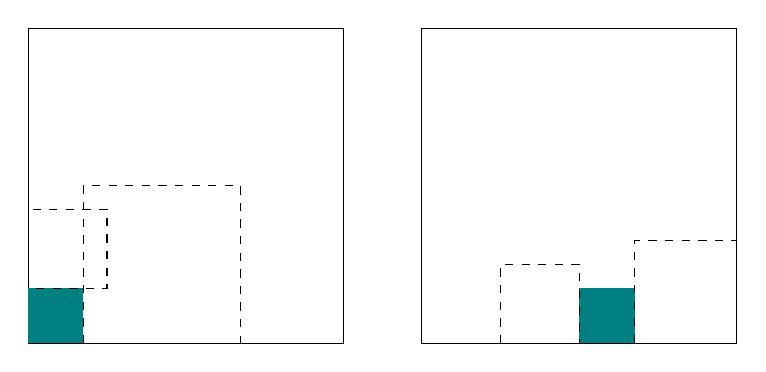
\begin{tikzpicture}
    % Első négyzet
    \draw (0,0) rectangle (4,4);
    \fill[teal](0, 0) rectangle (0.7, 0.7);
    \draw[dashed] (0, 0.7) rectangle (1, 1.7);
    \draw[dashed] (0.7, 0) rectangle (2.7, 2);

    % Második négyzet
    \draw (5,0) rectangle (9,4);
    \fill[teal](7, 0) rectangle (7.7, 0.7);
    \draw[dashed] (6, 0) rectangle (7, 1);
    \draw[dashed] (7.7, 0) rectangle (9, 1.3);
\end{tikzpicture} 
\par\end{center}
Ezt felhasználva tegyük fel, hogy az eredeti $a$ ($a\in\mathbb{N}^{+}$)
oldalú $K$ kockát sikerült felosztani különböző $a_{i}$ ($a_{i}\in\mathbb{N}^{+}$,
$i\in\mathbb{N}^{+}$) élű $K_{i}$ kis kockákra. Tekintsük ezután
$K$ egyik $L$ lapját! Az $L$-re illeszkedő kis kockák ezt a lapot
különböző méretű négyzetekre bontják. Legyen ezek közül a legkisebb
$N_{1}$, a hozzá tartozó kis kocka pedig $K_{1}$. Ekkor $N_{1}$
egyik oldala sem illeszkedik $L$ határoló vonalára, így az nagyobb
méretű négyzetekkel van körülvéve. Az ezekhez tartozó kis kockák olyan
üreget formálnak, amelyben helyezkedik el $K_{1}$. Legyen $K_{1}$-nek
$N_{1}$-gyel szemközti lapja $L_{1}$. Ekkor az $L_{1}$-re illeszkedő
kis kockák lapjai is felosztják $N_{1}$-et kisebb négyzetekre, melyek
közül a legkisebbet jelöljük $N_{2}$-vel. Ennek oldalára teljesül,
hogy $a_{2}<a_{1}$ ($a_{i}\in\mathbb{N}^{+}$), és $N_{2}$ $N_{1}$
belsejében helyezkedik el. Az $N_{2}$-t közrefogó nagyobb négyzetekhez
tartozó kockák ismét egy üreget formálnak, amelyben elhelyezkedik
$K_{2}$. Az eljárás $N_{2}$-vel szemben lévő $L_{2}$ lappal folytatva
olyan $(K_{m})$ sorozatot hozhatunk létre, melyek $(a_{n})$ él-sorozatára
$a>a_{1}>a_{2}>a_{3}>\dots$ ($a_{i}\in\mathbb{N}^{+}$, $i\in\mathbb{N}^{+}$).
Ez pedig a végtelen leszállás módszere alapján nem lehetséges, így
a kívánt kocka-felbontás nem végezhető el. 
\end{solution}
\begin{problem}
Adott a síkban $n$ darab kör. Bizonyítsuk be, hogy ezek bármilyen
egymáshoz viszonyított helyzete mellett az általuk alkotott „térkép”
kiszínezhető két színnel úgy, hogy az egymással szomszédos (közös
határvonallal rendelkező) tartományok eltérő színűek legyenek. 
\end{problem}

\begin{solution}
Matematikai indukcióval igazoljuk. Az $n=1$ eset egyértelmű: egyetlen
kör csak két tartományt (kör belseje és külseje) határol le, amely
egyszerűen 2 színnel színezhető.\\[6pt] \emph{Indukciós lépés}: Tegyük
fel, hogy bármely $n$ kör által alkotott térkép két színnel helyesen
színezhető. Vegyük el (távolítsuk el) az egyik kört, és színezzük
ki a maradék $n$ kör metszéshalmazait (ld.\ \textbf{A. ábra}). Ha
ez kész, tegyük vissza a $(n+1)$-edik kört, s a kör belsejében található
tartományokat (az új metszeteket) színezzük át a „másik” színre (ld.\ \textbf{B.
ábra}). Így megmarad a helyes kétszínezés. Ezzel készen vagyunk: teljes
indukcióval beláttuk az állítást. \quad{}

\vspace{1em}
\begin{center}
\begin{minipage}[c]{0.45\textwidth}%
\begin{tikzpicture}[scale=1, line cap=round, line join=round]
  %
  % Három kör definiálása:
  %   cA: r=1.0,  középpont (0,0)
  %   cB: r=1.5,  középpont (1.2,0)
  %   cC: r=2.0,  középpont (0.6,1.8)
  %
  \path[name path=cA] (0,0) circle (1.0);
  \path[name path=cB] (1.2,0) circle (1.5);
  \path[name path=cC] (0.6,1.8) circle (2.0);

  % -- Páros metszetek: színezzük világosabb szürkével (teal) --


  \begin{scope}
    \clip (0,0) circle (1.0);
    \fill[teal] (1.2,0) circle (1.5);
  \end{scope}

  
  \begin{scope}
    \clip (0,0) circle (1.0);
    \fill[teal] (0.6,1.8) circle (2.0);
  \end{scope}

 
  \begin{scope}
    \clip (1.2,0) circle (1.5);
    \fill[teal] (0.6,1.8) circle (2.0);
  \end{scope}

 
  \begin{scope}
    \clip (0,0) circle (1.0);
    \clip (1.2,0) circle (1.5);
    \fill[white] (0.6,1.8) circle (2.0);
  \end{scope}


  \draw (0,0) circle (1.0);
  \draw (1.2,0) circle (1.5);
  \draw (0.6,1.8) circle (2.0);

  % Felirat
  \node at (0.9, -2.2) {\small \textbf{A. ábra}};
\end{tikzpicture} %
\end{minipage}\hspace{0.05\textwidth} %
\begin{minipage}[c]{0.45\textwidth}%
\begin{tikzpicture}[scale=1, line cap=round, line join=round]
  %
  % Négy kör definiálása:
  %   cA: r=1.0,  középpont (0,0)
  %   cB: r=1.5,  középpont (1.2,0)
  %   cC: r=2.0,  középpont (0.6,1.8)
  %   cD: r=1.5,  középpont (-0.4,-0.2) (extra kör cA köré)
  %
  \path[name path=cA] (0,0) circle (1.0);
  \path[name path=cB] (1.2,0) circle (1.5);
  \path[name path=cC] (0.6,1.8) circle (2.0);
  \path[name path=cD] (-0.4,-0.2) circle (1.5);

  % -- Páros metszetek: cA, cB, cC, cD => színezzük gray!30 --

 
  \begin{scope}
    \clip (0,0) circle (1.0);
    \fill[teal] (1.2,0) circle (1.5);
  \end{scope}

  
  \begin{scope}
    \clip (0,0) circle (1.0);
    \fill[teal] (0.6,1.8) circle (2.0);
  \end{scope}

  
  \begin{scope}
    \clip (0,0) circle (1.0);
    \fill[teal] (-0.4,-0.2)  circle (1.5);
  \end{scope}

 
  \begin{scope}
    \clip (1.2,0) circle (1.5);
    \fill[teal] (0.6,1.8) circle (2.0);
  \end{scope}

 
  \begin{scope}
    \clip (1.2,0) circle (1.5);
    \fill[teal] (-0.4,-0.2)  circle (1.5);
  \end{scope}

  
  \begin{scope}
    \clip (0.6,1.8) circle (2.0);
    \fill[teal] (-0.4,-0.2)  circle (1.5);
  \end{scope}

  

 
  \begin{scope}
    \clip (0,0) circle (1.0);
    \clip (1.2,0) circle (1.5);
    \fill[white] (0.6,1.8) circle (2.0);
  \end{scope}

 
  \begin{scope}
    \clip (0,0) circle (1.0);
    \clip (1.2,0) circle (1.5);
    \fill[white] (-0.4,-0.2)  circle (1.5);
  \end{scope}

  \begin{scope}
    \clip (0,0) circle (1.0);
    \clip (0.6,1.8) circle (2.0);
    \fill[white] (-0.4,-0.2)  circle (1.5);
  \end{scope}

  
  \begin{scope}
    \clip (1.2,0) circle (1.5);
    \clip (0.6,1.8) circle (2.0);
    \fill[white] (-0.4,-0.2)  circle (1.5);
  \end{scope}

  
  \begin{scope}
    \clip (0,0) circle (1.0);
    \clip (1.2,0) circle (1.5);
    \clip (0.6,1.8) circle (2.0);
    \fill[teal] (-0.4,-0.2)  circle (1.5);
  \end{scope}

  % -- Körök körvonalai --
  \draw (0,0) circle (1.0);
  \draw (1.2,0) circle (1.5);
  \draw (0.6,1.8) circle (2.0);
  \draw (-0.4,-0.2)  circle (1.5);

  % Felirat
  \node at (1.1, -2.2) {\small \textbf{B. ábra}};
\end{tikzpicture} %
\end{minipage}
\par\end{center}
\end{solution}
\begin{problem}
Meg lehet-e választani a $\pm1\pm2\pm\dots\pm105$ kifejezésben az
előjeleket úgy, hogy a kifejezés értéke éppen 2025 legyen? 
\end{problem}

\begin{solution}
Belátjuk, hogy a $\pm1\pm2\pm\dots\pm105$ kifejezésben az előjelek
megfelelő megválasztásával minden $-5565$ és $5565$ közötti páratlan
szám előállítható. Ha minden előjel negatív, akkor az összeg $-5565$,
ha mindegyik pozitív, akkor pedig $5565$.

Állításunkat indukcióval igazoljuk. Tudjuk már, hogy $-5565$ előállítható
ilyen módon. Belátjuk, hogy ha $u<5565$ szerepel az összegek között,
akkor szerepel az $u+2$ is. Tekintsük $u$ előállításában balról
az első negatív előjelet (mivel $u<5565$, ilyen van). Ha ez az előjel
az $1$ előtt áll, akkor azt pozitívra változtatva az összeg kettővel
nő. Ha $1$-nél nagyobb szám előtt áll, akkor ezt az előjelet pozitívra
és az eggyel kisebb szám előtti pozitív előjelet negatívra változtatva,
az összeg ismét kettővel nő, vagyis előállítottuk az $u+2$-t.

Természetesen egy szám több különböző alakban is előállhat. Az 2025
egy lehetséges felírása: 
\[
-1-2-3\dots-59+60+61+\dots+105.
\]
\end{solution}
\begin{problem}
(Fermat tétele) Bizonyítsd, hogy Ha $p$ prím, $n$ pedig tetszőleges
természetes szám, akkor $n^{p}-n$ osztható $p$-vel.
\end{problem}

\begin{solution}
\smallskip{}
\emph{Bizonyítás vázlata}: 
\begin{itemize}
\item Az állítás $n=0$-ra triviálisan igaz. 
\item Tegyük fel, hogy $k^{p}-k$ minden $k\le n$-re osztható $p$-vel,
és bizonyítsuk be ugyanezt $n+1$-re. 
\item Elemzéssel felírjuk $(n+1)^{p}-(n+1)$ a binomiális tétel alapján,
és az így kapott kifejezések mindegyikéről belátjuk, hogy $p$-vel
osztható. Részletesen: 
\[
(k+1)^{p}-(k+1)=\sum_{j=0}^{p}\binom{p}{j}k^{j}\cdot1^{p-j}\;-\;k\;-\;1,
\]
amelyben $\binom{p}{j}$ $p$-vel osztható $1\le j\le p-1$ esetén,
míg a „szélső” tagokat (például $k^{p}-k$) az indukciós feltevés
fedezi. 
\item Ezzel a teljes indukció biztosítja, hogy $n^{p}-n$ tényleg osztható
$p$-vel minden $n$-re. 
\end{itemize}
\end{solution}
\begin{problem}
\emph{(Harmonikus, mértani és számtani közép tétele)}

Legyen $a_{1},a_{2},\dots,a_{n}$ tetszőleges pozitív valós szám.
Igazoljuk, hogy 
\[
\frac{n}{\frac{1}{a_{1}}+\frac{1}{a_{2}}+\cdots+\frac{1}{a_{n}}}\;\;\le\;\;\sqrt[n]{\,a_{1}a_{2}\cdots a_{n}\,}\;\;\le\;\;\frac{a_{1}+a_{2}+\cdots+a_{n}}{n},
\]
és az egyenlőség pontosan akkor teljesül, ha az összes $a_{i}$ megegyezik. 
\end{problem}

\begin{solution}
A következő, szép és nem szokványos \emph{indukciós} bizonyítást Cauchy-nak
tulajdonítják (lásd~{[}7{]}). A fenti láncegyenlőtlés második részét
(a mértani és számtani közép közötti egyenlőtlenséget) írjuk fel a
következő alakban: 
\[
P(n):\quad a_{1}a_{2}\cdots a_{n}\;\;\le\;\;\Bigl(\tfrac{a_{1}+\cdots+a_{n}}{n}\Bigr)^{n}.
\]

\medskip{}

\noindent\textbf{Az alapeset:} $n=2$. 
\[
a_{1}a_{2}\;\;\le\;\;\Bigl(\tfrac{a_{1}+a_{2}}{2}\Bigr)^{2}\;\;\Longleftrightarrow\;\;(a_{1}-a_{2})^{2}\;\ge\;0,
\]
ami nyilván igaz.

\medskip{}

\noindent\textbf{Továbblépés (két lépésben):} 
\begin{itemize}
\item[(A)] $P(n)\;\Longrightarrow\;P(n-1).$ 
\item[(B)] $P(n)\text{ és }P(2)\;\Longrightarrow\;P(2n).$ 
\end{itemize}
Ha (A) és (B) is teljesül, akkor nyilván belátjuk minden $n$-re az
állítást.

\medskip{}

\noindent\textbf{(A) lépés bizonyítása.} Legyen 
\[
A\;:=\;\frac{1}{n-1}\,\sum_{k=1}^{n-1}a_{k}.
\]
Ekkor a feltevés szerint ($P(n)$): 
\[
\Bigl(\prod_{k=1}^{n-1}a_{k}\Bigr)\,\cdot\,A\;\;\le\;\;\Bigl(\frac{\sum_{k=1}^{n-1}a_{k}+A}{n}\Bigr)^{n}.
\]
De $\sum_{k=1}^{n-1}a_{k}+A=(n-1)\,A+A=n\,A$, így a jobb oldal $(n\,A)^{n}/n^{n}=A^{n}$.
Tehát 
\[
\prod_{k=1}^{n-1}a_{k}\;\le\;A^{\,n-1}.
\]
Vagyis 
\[
P(n)\;\Longrightarrow\;\prod_{k=1}^{n-1}a_{k}\,\le\,A^{n-1},
\]
ami pontosan a $\prod_{k=1}^{n-1}a_{k}\le\Bigl(\frac{a_{1}+\cdots+a_{n-1}}{n-1}\Bigr)^{n-1}$
alak, azaz $P(n-1)$.

\medskip{}

\noindent\textbf{(B) lépés bizonyítása.} Most felhasználjuk $P(n)$
és $P(2)$ állítását a $2n$ darab $\{a_{1},\dots,a_{n},a_{n+1},\dots,a_{2n}\}$
számra. Írjuk szét: 
\[
\prod_{k=1}^{2n}a_{k}\;=\;\Bigl(\,\prod_{k=1}^{n}a_{k}\Bigr)\,\Bigl(\,\prod_{k=n+1}^{2n}a_{k}\Bigr).
\]
Először $P(n)$-t alkalmazzuk az elsõ $n$ tényezőre, majd $P(2)$-t
az így kapott számtani középre és a második $n$ tényező blokkra.
Az eredményként kapott kifejezés végül $\le$ 
\[
\Bigl(\frac{\sum_{k=1}^{2n}a_{k}}{2n}\Bigr)^{2n},
\]
ami éppen $P(2n)$. Ezzel (B) is igazolva van.

\medskip{}

\noindent Az egyenlőség feltételét (pontosan mikor lesz $\le$ helyett
$=$) a fenti lépésekben egyszerűen leolvashatjuk (minden lépésnél
$(a_{1}-a_{2})^{2}=0$-szerű feltételek). A harmonikus és a mértani
közép közti egyenlőtlenséget hasonló eljárással igazolhatjuk, ha a
$\bigl(a_{1},\dots,a_{n}\bigr)$ helyett a $\bigl(1/a_{1},\dots,1/a_{n}\bigr)$
sorozatot tekintjük. 
\end{solution}
\begin{problem}
Adott az $(a_{n})_{n\geq0}$ számsorozat, amelyre 
\begin{align*}
a_{0} & =1,\\
a_{0}+a_{1}+a_{2}+\dots+a_{n} & =a_{n}a_{n+1},\quad\forall n\in\mathbb{N}.
\end{align*}

(a) Határozd meg az $a_{1},a_{2},\dots,a_{10}$ értékét!\\
 (b) Határozd meg a sorozat általános tagját! \\
 (c) Bizonyítsd is be a kapott eredményt! \\
 \emph{(VII. OMMO, XXXIV. EMMV, megyei szakasz, XI. osztály, 2025. február 1.)}
 
\end{problem}

\begin{solution}
\textbf{Első megoldás}

(a) A rekurzió alapján: 
\begin{align*}
a_{0} & =a_{0}a_{1}\Rightarrow1=1\cdot a_{1}\Rightarrow a_{1}=1.
\end{align*}
Sorban kiszámolva: 
\begin{align*}
a_{0}+a_{1} & =a_{2}a_{1}\Rightarrow1+1=a_{2}\Rightarrow a_{2}=2,\\
a_{0}+a_{1}+a_{2} & =a_{3}a_{2}\Rightarrow1+1+2=2a_{3}\Rightarrow a_{3}=2,\\
a_{0}+a_{1}+a_{2}+a_{3} & =a_{4}a_{3}\Rightarrow1+1+2+2=2a_{4}\Rightarrow a_{4}=3,\\
\vdots\\
a_{0}+a_{1}+\dots+a_{9} & =a_{10}a_{9}\Rightarrow1+1+2+2+3+3+4+4+5+5=5a_{10}\Rightarrow a_{10}=6.
\end{align*}

(b) Az előző alpont alapján azt sejtjük, hogy $a_{2k}=a_{2k+1}=k+1$.
Matematika indukcióval igazoljuk.

Tegyük fel, hogy $a_{2k}=a_{2k+1}=k+1$. Indukcióval belátjuk, hogy:
\begin{align*}
a_{0}+a_{1}+\dots+a_{2k+1} & =a_{2k+2}a_{2k+1}.
\end{align*}
Mivel a bal oldal egy számtani sorozat összege, 
\begin{align*}
\frac{(k+1)(k+2)}{2}+(k+1) & =(k+1)a_{2k+2},
\end{align*}
és így egyszerűsítve: 
\begin{align*}
a_{2k+2} & =k+2.
\end{align*}
Ez teljes indukcióval igaz minden $n\in\mathbb{N}$ esetén.

\textbf{Megjegyzés:} Az általános tag alakja $a_{n}=\left\lceil \frac{n}{2}\right\rceil +1$. 
\end{solution}
%
\begin{solution}
\textbf{Második megoldás}

(a) A rekurzió alapján ugyanazokat az értékeket kapjuk. Átalakítjuk
az eredeti összefüggést: 
\begin{align*}
a_{n+1} & =\frac{a_{0}+a_{1}+\dots+a_{n}}{a_{n}}+1.
\end{align*}
Ez azt adja, hogy 
\begin{align*}
a_{n+1}=a_{n}+1,\quad\forall n\in\mathbb{N}.
\end{align*}
A kezdeti értékekből következik, hogy $a_{n}=\left\lceil \frac{n}{2}\right\rceil +1$.

(b) Indukcióval igazoljuk a sejtést: 
\begin{align*}
P(k):\quad a_{k}=\left\lceil \frac{k}{2}\right\rceil +1.
\end{align*}
Ellenőrizzük $P(0)$ és $P(1)$ esetén, majd felhasználva $P(k)$
igazságát, belátjuk, hogy $P(k+2)$ is igaz: 
\begin{align*}
a_{k+2} & =\left\lceil \frac{k+2}{2}\right\rceil +1.
\end{align*}
Ez teljes indukcióval igazolható, tehát 
\begin{align*}
a_{n}=\left\lceil \frac{n}{2}\right\rceil +1,\quad\forall n\in\mathbb{N}.
\end{align*}
\end{solution}
\begin{problem}
Legyen az $(x_{n})_{n\geq1}$ sorozat, amelyre 
\begin{align*}
x_{1} & =\frac{1}{4},\\
\sqrt{x_{n+1}}+\sqrt{x_{n}} & =\frac{2}{n^{2}+2n},\quad n\geq1.
\end{align*}
Bizonyítsuk be, hogy 
\begin{align*}
\sum_{k=1}^{n}(2k+1)x_{k}<1,\quad\forall n\geq1.
\end{align*}
\emph{(OMMO, helyi szakasz, Dolj megye, IX. osztály, 2020. február 8. )}
\end{problem}

\begin{solution}
Matematikai indukcióval bizonyítjuk, hogy 
\begin{align*}
x_{n}=\frac{1}{n^{2}(n+1)^{2}},\quad\forall n\geq1.
\end{align*}

\textbf{Bázislépés:} 
\begin{align*}
x_{1}=\frac{1}{4}=\frac{1}{1^{2}(1+1)^{2}},\quad\text{ami igaz.}
\end{align*}

\textbf{Indukciós lépés:} Tegyük fel, hogy 
\begin{align*}
x_{n}=\frac{1}{n^{2}(n+1)^{2}}
\end{align*}
és bizonyítsuk be, hogy 
\begin{align*}
x_{n+1}=\frac{1}{(n+1)^{2}(n+2)^{2}}.
\end{align*}

Az egyenletből: 
\begin{align*}
\sqrt{x_{n+1}}=\frac{2}{n^{2}+2n}-\sqrt{x_{n}}.
\end{align*}
Felhasználva az indukciós feltételt: 
\begin{align*}
\sqrt{x_{n}}=\frac{1}{(n+1)(n+1)},
\end{align*}
kapjuk, hogy 
\begin{align*}
\sqrt{x_{n+1}}=\frac{2}{n^{2}+2n}-\frac{1}{(n+1)(n+1)}=\frac{1}{(n+1)(n+2)}.
\end{align*}
Ezért: 
\begin{align*}
x_{n+1}=\frac{1}{(n+1)^{2}(n+2)^{2}}.
\end{align*}

Mivel mindkét lépés teljesült, az indukció elve szerint: 
\begin{align*}
x_{n}=\frac{1}{n^{2}(n+1)^{2}},\quad\forall n\geq1.
\end{align*}

Most bizonyítjuk a megadott összeg egyenlőtlenségét: 
\begin{align*}
\sum_{k=1}^{n}(2k+1)x_{k}=\sum_{k=1}^{n}(2k+1)\cdot\frac{1}{k^{2}(k+1)^{2}}.
\end{align*}
Felbontva: 
\begin{align*}
\sum_{k=1}^{n}\left(\frac{1}{k^{2}}-\frac{1}{(k+1)^{2}}\right).
\end{align*}
Ez egy teleszkopikus összeg, amelyből marad: 
\begin{align*}
1-\frac{1}{(n+1)^{2}}<1.
\end{align*}
Ezzel az állítás bizonyítva. 
\end{solution}

\section*{Nehezebb feladatok}
\begin{extraproblem}[Csapó Hajnalka]
Bizonyítsuk be, hogy minden háromszög felbontható $n$ darab hozzá
hasonló háromszögre, ha $n\geq6$. 
\end{extraproblem}

\begin{solution}
Ha egy háromszögben felvesszük az oldalak felezőpontjait és meghúzzuk
a középvonalakat, négy darab az eredetivel hasonló háromszög keletkezik.
Ez azt jelenti, hogy ha egy háromszöget felbontottunk $n$ darab vele
hasonló háromszögre, akkor a felbontás valamelyik háromszögét négy
háromszögre bontva, $n+3$ háromszögre is felbonthatjuk.
\begin{center}
\includegraphics[width=0.8\textwidth]{\string"content/Boga_Zsombor/indukcio1\string".png} 
\par\end{center}
A mellékelt ábrákon látható egy-egy felbontás $n=6$ illetve $n=8$
háromszögre. Mivel $7=4+3$ háromszögre is felbonthatjuk és így az
első észrevétel és a teljes indukció elve alapján szerkeszthetünk
minden $n\geq6$ esetén olyan felbontást, amely $n$ darab az eredetivel
hasonló háromszöget tartalmaz.
\end{solution}
\begin{extraproblem}[Csapó Hajnalka]
Feldarabolható-e egy általános háromszög $n$ darab egyenlő szárú
háromszögre, ha $n\geq4$? 
\end{extraproblem}

\begin{solution}
~
\begin{center}
\includegraphics[width=0.5\textwidth]{\string"content/Boga_Zsombor/indukcio2\string".png} 
\par\end{center}
Ha egy derékszögű háromszögben meghúzzuk a derékszöghöz tartozó oldalfelezőt,
két egyenlő szárú háromszög keletkezik. Mivel minden háromszögnek
van legalább egy olyan magassága, amely a háromszög belsejében van,
minden háromszög felbontható 4 egyenlő szárú háromszögre. Ez egyben
azt is jelenti, hogy ha van felbontás $n$ háromszögre, akkor van
$n+3$ háromszögre is. Ugyanakkor ha előbb levágunk egy vagy két egyenlő
szárú háromszöget, akkor kaphatunk 5 illetve 6 háromszöget tartalmazó
felbontást is. Így tetszőleges $n\geq4$ esetén szerkeszthetünk $n$
darab egyenlő szárú háromszöget tartalmazó felbontást. (Ha ez a háromszög
egyenlő szárú, akkor az előbbi feladatot is használhatjuk.) 
\end{solution}
\begin{extraproblem}[Czofa Vivien]
\textit{\emph{Határozzuk meg azon $f:\mathbb{N}^{+}\to\mathbb{N}^{+}$
függvényeket, amelyek esetén teljesül az}}\emph{ 
\[
f(1)-2f(2)+3f(3)-4f(4)+\dots+(-1)^{n-1}nf(n)=\frac{(-1)^{n-1}nf(n+1)}{2}
\]
}\textit{\emph{egyenlőség, bármilyen $n\in\mathbb{N}^{+}$ esetén.
}}\textit{(Matematika Olimpia, Helyi szakasz, Suceava, 2016)}
\end{extraproblem}

\begin{solution}
Legyen $f(1)=a\in\mathbb{N}^{+}$. Ekkor $n=1$-re azt kapjuk, hogy
\[
f(1)=\frac{f(2)}{2}\iff f(2)=2a.
\]

Ha $n=2$-t helyettesítünk az egyenlőségbe, kapjuk, hogy 
\[
f(3)=3a.
\]

Ezek alapján megfogalmazható egy sejtés, mely szerint $f(n)=an$,
$\forall a,b\in\mathbb{N}^{+}$ esetén, amit a matematikai \textit{indukció}
módszerével igazolunk.

Láthatjuk, hogy az állítás $n=1$ és $n=2$ esetén valóban teljesül.
Feltételezzük, hogy $f(n)=an$, $\forall a,b\in\mathbb{N}^{+}$, és
bebizonyítjuk, hogy $f(n+1)=a(n+1)$, $\forall a,b\in\mathbb{N}^{+}$.

A feladat kijelentésében szereplő egyenlőséget felírva $n-1$ illetve
$n$ tagra kapjuk az 
\[
f(1)-2f(2)+3f(3)-4f(4)+\dots+(-1)^{n-2}(n-1)f(n-1)=\frac{(-1)^{n-2}(n-1)f(n)}{2}
\]
és az 
\[
f(1)-2f(2)+3f(3)-4f(4)+\dots+(-1)^{n-1}nf(n)=\frac{(-1)^{n-1}nf(n+1)}{2}
\]
egyenlőségeket, amelyeket kivonva egymásból kapjuk, hogy 
\[
nf(n+1)=(n+1)f(n),\quad\forall n\in\mathbb{N}^{+}.
\]

Felhasználva az indukciós feltevésünket, mely szerint $f(n)=an$ következik,
hogy $f(n+1)=a(n+1)$, $\forall n\in\mathbb{N}^{+}$. Tehát a matematikai
indukció módszere alapján igazoltuk, hogy $f(n)=an$, $\forall n\in\mathbb{N}^{+}$
esetén, így a keresett függvények az $f:\mathbb{N}^{+}\to\mathbb{N}^{+}$,
$f(n)=an$, $a\in\mathbb{N}^{+}$ alakú függvények.
\end{solution}
\begin{extraproblem}[Czofa Vivien]
\textit{\emph{Határozzátok meg azokat az $f:\mathbb{N}^{*}\rightarrow\mathbb{R}$
függvényeket, amelyek rendelkeznek a következő tulajdonsággal:}}\emph{
\[
f(1)+2\cdot f(2)+3\cdot f(3)+\dots+n\cdot f(n)=f(n+1)-1,\quad\forall n\in\mathbb{N}^{*}.
\]
}

\textit{(Matematika Tantárgyverseny, Bihar megye, 2020, IX. osztály)}
\end{extraproblem}

\begin{solution}
$n=1\Longrightarrow f(2)=1+f(1);$

$n=2\Longrightarrow f(1)+2f(2)=3(1+f(1))=\frac{3!}{2}(1+f(1));$

$n=3\Longrightarrow f(1)+2f(2)+3f(3)=12(1+f(1))=\frac{4!}{2}(1+f(1)).$

\textbf{Sejtés:} $f(n)=\frac{n!}{2}(1+f(1))$, $\forall n\geq2$.
\textbf{Bizonyítás matematikai }\textbf{\textit{indukció}}\textbf{val:}

\textbf{I.} $k=2$-re igaz: 
\[
f(2)=\frac{2!}{2}(1+f(1))=1+f(1)
\]

\textbf{II.} Feltételezzük, hogy $k$-ig igaz, és bizonyítjuk $k+1$-re:

\begin{align*}
f(k+1) & =f(1)+2f(2)+3f(3)+\dots+kf(k)+1\\
 & =\frac{2!}{2}(1+f(1))+\frac{3!}{2}(1+f(1))+\dots+\frac{k!}{2}(1+f(1))\\
 & =\left(\frac{2!+3!+\dots+k!}{2}\right)(1+f(1))\\
 & =\left(\frac{(k+1)!-2}{2}\right)(1+f(1))\\
 & =\frac{(k+1)!}{2}(1+f(1)),\quad\forall k\geq2.
\end{align*}

Ahol felhasználtuk, hogy 
\[
1\cdot1!+2\cdot2!+3\cdot3!+\dots+k\cdot k!=(k+1)!-1.
\]

\textbf{Jelöljük} $f(1)=a$, ahol $a\in\mathbb{R}$. Ekkor a keresett
függvény: 
\[
f:\mathbb{N}^{*}\to\mathbb{R},\quad f(n)=\begin{cases}
a, & n=1;\\
\frac{n!}{2}(1+a), & n\geq2.
\end{cases}
\]
\end{solution}
\begin{extraproblem}[Fábián Nóra]
Határozd meg az $\left\lfloor \frac{n}{\sqrt[k]{n!}}\right\rfloor $
szám egész részét, ha $n\geq6$.
\end{extraproblem}

\begin{solution}
s$n=6$ esetén $\left\lfloor \frac{6}{\sqrt[6]{6!}}\right\rfloor =2$,
\quad{}$n=7$-re $\left\lfloor \frac{7}{\sqrt[7]{7!}}\right\rfloor =2$.
Sejtjük, hogy 
\[
\left\lfloor \frac{n}{\sqrt[k]{n!}}\right\rfloor =2\quad\text{minden }n\geq6
\]
esetén. Tekintjük a $P(n):\left\lfloor \frac{n}{\sqrt[k]{n!}}\right\rfloor =2$
kijelentést. $n\in\{6,7\}$ esetén ez a kijelentés igaz. Ha a kijelentés
igaz egy $k\geq6$ szám esetén, akkor 
\[
2<\frac{k}{\sqrt[k]{k!}}<3,
\]
ami egyenértékű a 
\[
2^{k}<\frac{k^{k}}{k!}<3^{k}
\]
egyenlőtlenségekkel. Tudjuk, hogy 
\[
\left(1+\frac{1}{k}\right)^{k}>2\quad\text{és}\quad\frac{k^{k}}{k!}>2^{k}.
\]
Összeszorozva az egyenlőtlenségek megfelelő oldalait az 
\[
\frac{(k+1)^{k}}{k^{k}}\cdot\frac{k^{k}}{k!}>2^{k+1}\iff\frac{(k+1)^{k+1}}{(k+1)!}>2^{k+1}\quad(1)
\]
egyenlőséget kapjuk. Ugyanakkor 
\[
\left(1+\frac{1}{k}\right)^{k}\leq3\quad\text{és}\quad\frac{k^{k}}{k!}\leq3^{k}.
\]
Ebből a két egyenlőtlenségből az 
\[
\frac{(k+1)^{k}}{k^{k}}\cdot\frac{k^{k}}{k!}\leq3^{k}\iff\frac{(k+1)^{k+1}}{(k+1)!}\leq3^{k+1}\quad(2)
\]
egyenlőséget kapjuk. Tehát (1), (2) alapján $2^{k+1}<\frac{(k+1)^{k+1}}{(k+1)!}\leq3^{k+1}$,
ahonnan $2<\frac{k+1}{(k+1)!^{\frac{1}{k+1}}}\leq3$, azaz $\Bigg[{\displaystyle {\frac{k+1}{(k+1)!^{\frac{1}{k+1}}}}\Bigg]=2}$.
Így a kijelentés $k+1$-re is igaz.
\end{solution}
\begin{extraproblem}[Csurka-Molnár Hanna]
Bizonyítsuk be, hogy $A=\begin{bmatrix}1 & 0\\
2 & 1
\end{bmatrix}$ mátrix esetén $A^{n}=n\cdot A-(n-1)\cdot I_{2}$ bármely $n\in\mathbb{N}^{*}$
esetén! 
\end{extraproblem}

\begin{solution}
$n=1$ esetén az összefüggés teljesül: $A^{1}=1\cdot A-(1-1)\cdot I_{2}=A$.

Feltételezzük, hogy $P(n):A^{n}=n\cdot A-(n-1)\cdot I_{2}$ igaz bármely
$n\leq k$ rögzített $k\in\mathbb{N}$ esetén. Ekkor 
\begin{align*}
A^{k} & =k\cdot A-(k-1)\cdot I_{2}\Rightarrow\\
\Rightarrow A^{k}\cdot A & =k\cdot A\cdot A-(k-1)\cdot I_{2}\cdot A\Rightarrow\\
\Rightarrow A^{k+1} & =k\cdot A^{2}-(k-1)\cdot A\Rightarrow\\
\end{align*}

A Cayley-Hamilton--tétel alapján tudjuk, hogy 
\begin{align*}
A^{2} & =\text{tr}(A)\cdot A-\det(A)\cdot I_{2}\\
A^{2} & =(1+1)\cdot A-(1\cdot1-2\cdot0)\cdot I_{2}\\
A^{2} & =2\cdot A-I_{2}\,.
\end{align*}

A fenti összefüggések alapján 
\begin{align*}
A^{k+1} & =k\cdot\left[2\cdot A-I_{2}\right]-(k-1)\cdot A\\
A^{k+1} & =2k\cdot A-k\cdot I_{2}-k\cdot A+A\\
A^{k+1} & =k\cdot A+A-k\cdot I_{2}\\
A^{k+1} & =(k+1)\cdot A-\left[(k+1)-1\right]\cdot I_{2}\\
\end{align*}
tehát $P(k+1)$ is igaz.

Mivel $P(1)$ igaz és feltételezve, hogy $P(k)$ igaz, következtettünk
arra, hogy $P(k+1)$ is igaz, a matematikai indukció alapján $P(n)$
igaz $\forall n\in\mathbb{N}$.
\end{solution}
\begin{extraproblem}[Csurka-Molnár Hanna]
Hányféleképpen írhatjuk fel a 2015-öt néhány (egy vagy több) pozitív
egész szám összegeként, ha az összeadandók sorrendje is számít? 
\end{extraproblem}

\begin{solution}
Próbálkozzunk először a 2015 helyett kisebb számokkal. Az 1-et 1-féleképpen
írhatjuk fel (1), a 2-t 2-féleképpen $(2=1+1)$, a 3 -at 4 -féleképpen
$(3=1+2=2+1=1+1+1)$. Innen megsejthetjük, hogy az $n$ pozitív egész
szám lehetséges felírásainak száma $2^{n-1}$.

Sejtésünket teljes indukcióval igazoljuk. Az állítás a fent látott
módon igaz $n=1,2$, 3-ra. Tegyük fel most, hogy az állítás igaz valamilyen
rögzített $k$-ra, majd lássuk be $k+1$-re. Tudjuk tehát, hogy a
$k$ pozitív egész számot $2^{k-1}$-féle összegként írhatjuk fel,
és ennek segítségével be szeretnénk látni, hogy a $k+1$ számot $2^{k}$-féleképpen
(vagyis kétszer annyi módon) írhatjuk fel.

Tekintsük a $k$ szám összegként történő felírásait. Minden ilyen
felírásból képezhetjük a $k+1$ szám két különböző felírását: az egyiket
úgy, hogy az utolsó összeadandót 1-gyel növeljük, a másikat pedig
úgy, hogy még egy +1 tagot az összeg végére írunk. (Például $k=2$
esetén a 2 -ből kapjuk így a 3 és a $2+1$ felírásokat, míg az $1+1$-ből
az $1+2$ és az $1+1+1$ felírásokat.) Így a $k$ szám $2^{k-1}$
különböző felírásából a $k+1$ szám $2\cdot2^{k-1}=2^{k}$ db felírását
kaptuk. Ezek mind különbözőek, továbbá a $k+1$ szám tetszőleges felírása
előáll így, hiszen az eljárás visszafelé is egyértelmű (a $k+1$ szám
egy adott felírásából megkaphatjuk a $k$ szám egy felírását úgy,
hogy ha az utolsó öszszeadandó 1 , akkor ezt elhagyjuk, ellenkező
esetben pedig 1-gyel csökkentjük). Tehát a $k+1$ számra $2^{k}$
lehetséges felírást kaptunk, ezzel az indukciós lépést beláttuk.

Vagyis a 2015-öt $2^{2014}$-féleképpen írhatjuk fel néhány pozitív
egész összegeként. 
\end{solution}
\begin{extraproblem}[Csurka-Molnár Hanna]
Hány olyan 150-jegyű tízes számrendszerbeli pozitív egész szám van,
amelynek minden számjegye páratlan, és bármely két szomszédos jegy
eltérése 2 ? (OKTV 2013/2014; II. kategória, 2. forduló) 
\end{extraproblem}

\begin{solution}
A feladatot először kevesebb jegyű számokra vizsgáljuk meg. Tekintsük
azokat az n-jegyű tízes számrendszerbeli pozitív egészeket, amelyeknek
minden számjegye páratlan, és bármely két szomszédos jegy eltérése
2. Jelölje ezek közül az 1-re vagy 9-re végződők számát $a_{n}$,
a 3-ra vagy 7-re végződők számát $b_{n}$, az 5-re végződők számát
pedig $c_{n}$. Feladatunk $a_{150}+b_{150}+c_{150}$ meghatározása.
Tudjuk, hogy $n=1$ esetén $a_{1}=2,b_{1}=2$ és $c_{1}=1$.

Mivel $n+1$-jegyű 1-re vagy 9-re végződő számot csak egyféleképpen
kaphatunk ( $n$-jegyű 3-ra vagy 7-re végződő számból), ezért $a_{n+1}=b_{n}$.
Ez igaz az 5-re végződőkre is, így $c_{n+1}=b_{n}$. Mivel 3ra vagy
7 -re végződő számot egyféleképpen kaphatunk 1-re vagy 9-re végződő
számból, de kétféleképpen kaphatunk 5-re végződőből (az 5 után 3-at
vagy 7-et írhatunk), ezért $b_{n+1}=a_{n}+2c_{n}$. Ebből $n=2$-re
az $a_{2}=2,b_{2}=4$ és $c_{2}=2$ értékeket kapjuk. (A megfelelő
számok: 31, 79 / 13, 53, 57, 97 / 35, 75.)

Írjuk fel a rekurzió segítségével a sorozatok első néhány értékét:
\begin{center}
\begin{tabular}{|c|c|c|c|c|c|c|}
\hline 
$n$ & 1 & 2 & 3 & 4 & 5 & 5\tabularnewline
\hline 
$a_{n}$ & 2 & 2 & 4 & 6 & 12 & 18\tabularnewline
\hline 
$b_{n}$ & 2 & 4 & 6 & 12 & 18 & 36\tabularnewline
\hline 
$c_{n}$ & 1 & 2 & 4 & 6 & 12 & 18\tabularnewline
\hline 
\end{tabular}
\par\end{center}
Az első néhány elemből megsejthetjük, hogy $a_{2n}=c_{2n}=2\cdot3^{n-1}$
és $b_{2n}=4\cdot3^{n-1}$. A sejtést teljes indukcióval bizonyítjuk,
$n=1$-re a sorozatok megfelelő elemeinek kiszámolásával már beláttuk.

Tegyük fel tehát, hogy valamely n-re $a_{2n}=c_{2n}=2\cdot3^{n-1}$
és $b_{2n}=4\cdot3^{n-1}$ teljesül, majd ennek segítségével lássuk
be az állítást $n+1$-re is. A következő sorok mindegyikében az első
két egyenlőségnél a rekurzív összefüggést, a harmadiknál az indukciós
feltevést használjuk:

\[
\begin{aligned} & a_{2(n+1)}=c_{2(n+1)}=b_{2n+1}=a_{2n}+2c_{2n}=2\cdot3^{n-1}+4\cdot3^{n-1}=2\cdot3^{n}\\
 & b_{2(n+1)}=a_{2n+1}+2c_{2n+1}=b_{2n}+2b_{2n}=4\cdot3^{n-1}+8\cdot3^{n-1}=4\cdot3^{n}
\end{aligned}
\]

Ezzel a sejtést beláttuk, így $a_{150}+b_{150}+c_{150}=2\cdot3^{74}+4\cdot3^{74}+2\cdot3^{74}=8\cdot3^{74}$.
Tehát $8\cdot3^{74}$ darab 150-jegyű szám teljesíti a feladat feltételeit.

Megjegyzés: Bár a feladatban az $a_{n},b_{n},c_{n}$ sorozatoknak
csak a páros indexű tagjait használjuk, hasonló módon adható zárt
képlet a páratlan indexűekre is: minden pozitív egész $n$ szám esetén
$a_{2n+1}=c_{2n+1}=4\cdot3^{n-1}$ és $b_{2n+1}=2\cdot3^{n}$.
\end{solution}
\begin{extraproblem}[Gergely Verona]
Bizonyítsuk be, hogy minden pozitív egész $n$ esetén $2^{4n}-1$
és $2^{4n}+1$ közül valamelyik osztható $17$-tel. \emph{(KöMaL,
2009) }
\end{extraproblem}

\begin{solution}
Ha $n=1$ akkor $2^{4}+1=17$, osztható $17$-tel. Ha $n=2$ akkor
$2^{8}-1=(2^{4}+1)(2^{4}-1)=17\cdot15$, osztható $17$-tel. \\

Sejtés: ha $n$ páratlan, akkor $17$ osztója $2^{4n}-1$-nek, ha
pedig páros, akkor osztója $2^{4n}+1$-nek. \\

Bizonyítás teljes indukcióval:\\

Legyen $n=2k+1$ ($k=0,1,2,\dots$). Igazoltuk, hogy $n=1$-re igaz
az állítás.

Feltételezzük , hogy $n=(2k+1)$-re is igaz, azaz 
\[
2^{4(2k+1)}+1=2^{8k+4}+1=17\cdot x,
\]
ahol $x$ egész. Belátjuk, hogy akkor $n=2(k+1)+1$-re is igaz, vagyis
a tulajdonság öröklődik.

\begin{align*}
2^{4[2(k+1)+1]}+1 & =2^{8k+4}\cdot2^{8}+1\\
 & =(17x-1)\cdot2^{8}+1\\
 & =17\cdot256\cdot x-256+1\\
 & =17\cdot256\cdot x-17\cdot15,
\end{align*}

ami osztható $17$-tel.

Legyen most $n=2k$ ($k=1,2,3,\dots$).Igazoltuk, hogy $n=2$-re igaz
az állítás. Feltételezzük, hogy $n=2k$-ra is igaz: 
\[
2^{4n}-1=2^{8k}-1=17\cdot y,
\]
és legyen $n=2(k+1)$, ekkor

\begin{align*}
2^{4(2(k+1))}-1 & =2^{8k}\cdot2^{8}-1\\
 & =(17y+1)\cdot2^{8}-1\\
 & =17\cdot256\cdot y+17\cdot15.
\end{align*}

Valóban, ez is osztható $17$-tel.

Ezzel a bizonyítást befejeztük. 
\end{solution}
\begin{extraproblem}[Kis Aranka-Enikő]
Határozzuk meg az összes olyan $f:\mathbb{N^{*}}\to\mathbb{N}$ függvényt,
amely teljesíti a következő feltételeket:
\end{extraproblem}

\begin{enumerate}
\item[(a)] $f(a\cdot b)=f(a)\cdot f(b),\quad\forall a,b\in\mathbb{N}$
\item[(b)] Ha $a<b$, akkor $f(a)<f(b)$
\item[(c)] $f(2)=2$
\end{enumerate}
\begin{solution}
Az (a) összefüggésbe $a=b=1$-et helyettesítve: 
\[
f(1)=f(1)\cdot f(1)\Rightarrow f(1)=1.
\]

A (c) feltétel alapján $f(2)=2$. Ha az (a) összefüggésbe $a=b=2$-t
helyettesítünk: 
\[
f(4)=f(2)\cdot f(2)=4.
\]

A (b) feltétel alapján, mivel $2<3<4$, következik, hogy: 
\[
f(2)<f(3)<f(4),
\]
\[
2<f(3)<4.
\]

Mivel $2$ és $4$ között egyetlen természetes szám található, a $3$,
így: 
\[
f(3)=3.
\]

Észrevesszük, hogy $f(n)=n$ minden $n\in\{1,2,3,4\}$ esetén. Indukcióval
bizonyítjuk, hogy: 
\[
f(n)=n,\quad\forall n\in\mathbb{N}.
\]

Indukciós lépés:

Feltételezzük, hogy $P(k):f(k)=k$ igaz minden $k\leq n$ esetén.

Ha $n+1$ páros, akkor létezik olyan $k\leq n$, amelyre $n+1=2k$.
Innen: 
\[
f(n+1)=f(2k)=f(2)\cdot f(k)=2k=n+1.
\]

Ha $n+1$ páratlan, akkor létezik olyan $k$, amelyre $n+1=2k+1$.
Ekkor: 
\[
2k<n+1<f(n+1)<f(2k+2).
\]

De: 
\[
f(2k)=f(2)\cdot f(k)=2k,\quad\text{mivel }k\leq n,
\]
\[
f(2k+2)=f(2)\cdot f(k+1)=2k+2,\quad\text{mivel }k+1\leq n.
\]

Így: 
\[
2k<f(n+1)<2k+2,
\]

ahonnan $f(n+1)=2k+1=n+1$.

Tehát $f(n+1)=n+1$, ha $f(k)=k,\forall k\leq n$ esetén. Az 1.3.3.
tétel értelmében: 
\[
f(n)=n,\quad\forall n\in\mathbb{N}.
\]
\end{solution}
\begin{extraproblem}[Kiss Andrea-Tímea]
Igazoljuk, hogy $n$ egyenes a síkot legfeljebb $\dfrac{n^{2}+n+2}{2}$
részre osztja fel! 
\end{extraproblem}

\begin{solution}
Tekintsük a következő állítást: 
\[
P(n):n\text{ egyenes a síkot }\dfrac{n^{2}+n+2}{2}\text{ részre osztja, minden }n\in\mathbb{N}^{*}\text{ esetén.}
\]
$P(1)$ igaz, mivel egy egyenes a síkot két részre osztja és $2=\dfrac{1^{2}+1+2}{2}$.

Feltételezzük, hogy $P(k)$ igaz minden $k\in\mathbb{N}^{*}$ esetén.

A $(k+1)$-ik egyenes akkor osztja minél több részre a már $k$ egyenes
által létrehozott részeket, ha minden egyenest pontosan egy pontban
metszi, ugyanakkor ezek a metszéspontok páronként különbözőek, vagyis
nincs a $k+1$ egyenes között három összefutó, valamint egybeeső és
párhuzamos egyenesek sem.

Ekkor a $(k+1)$-ik egyenes a $k$ egyenest $k$ különböző pontban
metszi, illetve az újonnan berajzolt egyenes még a $(k+1)$ részt
két részre oszt.

Tehát 
\[
\begin{array}{l}
\dfrac{k^{2}+k+2}{2}+2(k+1)-(k+1)=\dfrac{k^{2}+k+2}{2}+k+1=\dfrac{k^{2}+k+2+2k+2}{2}=\\
=\dfrac{(k+1)^{2}+(k+1)+2}{2},\forall k\in\mathbb{N}^{*},
\end{array}
\]
ahonnan következik, hogy $P(k+1)$ igaz.

A matematikai indukció elve alapján következik, hogy $P(n)$ igaz
minden $n\in\mathbb{N}^{*}$ esetén. 
\end{solution}
\begin{extraproblem}[Miklós Dóra]
Igazoljuk, hogy $2^{1994}$-nek van olyan többszöröse, amelynek tízes
számrendszerbeli alakja csak az $1$-es és $2$-es számjegyeket tartalmazza!
\emph{(NMMV 1994) }
\end{extraproblem}

\begin{solution}
Előbb vizsgáljuk meg a feladatot kisebb hatványokra. Például $2^{1}$
esetén a $2$ egy megfelelő szám, hasonlóan $2^{2}$ esetén $12$
és $2^{3}$ esetén $112$. Valami képzési szabályra kellene rájönnünk
ezek alapján. Tudva, hogy $112=2^{3}\cdot14$ mit kellene hozzáadnunk,
hogy egy $2^{4}$-nel osztható számot kapjunk és a megjelenő számjegy
$1$-e vagy $2$-es legyen. Ha az ezresek helyére szeretnénk egy számjegyet
beilleszteni, akkor vagy $1000=2^{3}\cdot5^{3}$ vagy $2000=2^{3}\cdot2\cdot5^{3}$
adhatunk hozzá. Mivel a $112$ felírásában a $14$ páros ezért $2000$-et
kell hozzáadnunk, hogy $16$-tal oszthatóvá váljon, hiszen: 
\[
2112=112+2000=2^{3}\cdot14+2^{3}\cdot2\cdot5^{3}=2^{3}\cdot(14+250)=2^{3}\cdot264=2^{4}\cdot132.
\]
Sejthető, hogy hasonló szerkesztés mellett tetszőleges $n$-re tudunk
mondani olyan számot, mely osztható $2^{n}$-nel és számjegyeit $1$-esek
és $2$-esek alkotják. A sejtést matematikai indukcióval fogjuk igazolni.

Mint korábban beláttuk, $n\in\{1,2,3,4\}$ értékekre meg tudjuk adni
a megfelelő többszörösöket. A továbbiakban feltételezzük, hogy létezik
olyan $a_{n}$ szám, mely osztható $2^{n}$-nel és számjegyeit csak
$1$-esek és $2$-esek alkotják. Igazoljuk, hogy $n+1$-re is meg
tudjuk adni a megfelelő számot, mely legyen a következő: 
\begin{itemize}
\item ha $a_{n}$ nem osztható $2^{n+1}$-nel, akkor $a_{n+1}=a_{n}+10^{n}$; 
\item ha $a_{n}$ osztható $2^{n+1}$-nel, akkor $a_{n+1}=a_{n}+2\cdot10^{n}$. 
\end{itemize}
Ilyen megválasztás mellett $a_{n+1}$ valóban teljesíti a feltételeket.

Összesítve elmondható, hogy tetszőleges $n\geq1$ esetén megadható
olyan többszöröse a $2^{n}$-nek, melynek számjegyei $1$-esek és
$2$-esek. Így a $2^{1994}$ esetén is létezik ilyen szám.
\end{solution}
\begin{extraproblem}[Péter Róbert]
Igazoljuk, hogy ha egy pozitív egész szám $3^{n}$ egyforma számjegyből
áll, akkor ez a szám osztható $3^{n}$-nel.\\
 
\end{extraproblem}

\begin{solution}
\underline{1. alapeset: P(1) ($n=1$)}\\
 Az $n=1$ esetben a bizonyítandó állítás az,
hogy $x\cdot111$ osztható 3-mal, ahol $x$ egy nullától különböző
tetszőleges számjegy.

Ez az állítás nyilván igaz, mert a szám számjegyeinek összege:

\[
1+1+1=3,
\]

ami osztható 3-mal, így az egész szám is osztható 3-mal.

Ellenőrizhetjük az $n=2$ esetet is. Ekkor a vizsgált szám:

\[
x\cdot111111111
\]

A számjegyek összege:

\[
1+1+1+1+1+1+1+1+1=9,
\]

ami osztható 9-cel, tehát a szám valóban osztható $3^{2}=9$-cel.

\underline{2. Indukciós lépés}\\

Tegyük fel, hogy az állítás igaz minden $n\in\mathbb{N}$-re, azaz:

\[
P(n):\text{Minden }3^{n}\text{ egyforma számjegyből álló szám osztható }3^{n}\text{-nel.}
\]

\underline{3. Indukciós lépés ($n\to n+1$)}\\

Meg kell mutatnunk, hogy ha $P(n)$ igaz, akkor $P(n+1)$ is igaz.

A $P(n+1)$ állításban szereplő számot úgy kaphatjuk meg, hogy a $P(n)$
esetében lévő számot háromszor egymás után írjuk:

\[
x\cdot(\underbrace{111\ldots111}_{3^{n}\text{ db 1}})
\]

Az indukciós hipotézis szerint ez a szám osztható $3^{n}$-nel, tehát
létezik egy egész szám $A$, amelyre:

\[
x\cdot(\underbrace{111\ldots111}_{3^{n}\text{ db 1}})=3^{n}\cdot x\cdot A
\]

Ezzel a $P(n+1)$ esetében kapott szám így írható:

\[
x\cdot(\underbrace{111\ldots111}_{3^{n+1}\text{ db 1}})=3^{n}\cdot x\cdot(AAA)
\]

ahol $AAA$ az $A$ szám háromszoros ismétlése.

Egy szám pontosan akkor osztható $3^{n+1}$-gyel, ha osztható $3^{n}$-nel,
és az így kapott hányados még osztható 3-mal. Tehát már csak azt kell
belátnunk, hogy:

\[
x\cdot(AAA)
\]

osztható 3-mal. Ez nyilván teljesül, mivel az $AAA$ szám számjegyeinek
összege pontosan az $A$ szám számjegyeinek összegének háromszorosa,
és mivel $A$ osztható 3-mal, ez az összeg is osztható 3-mal.

Ezzel beláttuk, hogy ha az állítás igaz $n$-re, akkor igaz $n+1$-re
is, így a teljes indukció elve alapján az állítás minden pozitív egész
$n$-re igaz. 
\end{solution}
\begin{extraproblem}[Seres Brigitta-Alexandra]
Az $(a_{n})_{n\in\mathbb{N}}$ sorozatot a következőképpen értelmezzük:
\[
a_{0}=a_{1}=1\quad\text{és}\quad17^{a_{n+2}}=15^{a_{n+1}}+8^{a_{n}},\quad\forall n\in\mathbb{N}.
\]
a.) Igazold, hogy $(a_{n})_{n\in\mathbb{N}}$ sorozat konvergens!\\
 b.) Számítsd ki az $(a_{n})_{n\in\mathbb{N}}$ sorozat határértékét!
\begin{flushright}
\textit{ (OMMO(EMMV) 2024, XI. osztály, I. forduló, 1. feladat)} 
\par\end{flushright}
\end{extraproblem}

\begin{solution}
\textbf{a.)} Mivel $a_{0}=a_{1}=1$ és $17^{a_{2}}=15^{1}+8^{1}=23$,
következik, hogy $a_{2}=\log_{17}23>1$. Mivel $a_{0}\leq a_{1}<a_{2}$,
sejthető, hogy egy növekvő sorozatunk van. Ezen sejtést matematikai
indukcióval fogjuk belátni.

Valóban teljesül $a_{0}\leq a_{1}<a_{2}$. Feltételezzük, hogy $a_{k}\leq a_{k+1}$,
bármely $k=\overline{1,n-1}$ esetén, és belátjuk, hogy ekkor $a_{n}\leq a_{n+1}$
is teljesül. A feltevés szerint $a_{n-2}\leq a_{n-1}$ és $a_{n-1}\leq a_{n}$.
Ugyanakkor tudjuk, hogy $f(x)=15^{x}$ és $g(x)=8^{x}$ növekvő függvények,
így az indukciós feltevést is figyelembe véve, igaz hogy 
\[
8^{a_{n-2}}+15^{a_{n-1}}\leq8^{a_{n-1}}+15^{a_{n}},
\]
ami a rekurzió értelmezése szerint ekvivalens azzal, hogy 
\[
17^{a_{n}}\leq17^{a_{n+1}}.
\]
Ugyanakkor $h(x)=17^{x}$ is növekvő függvény, így $17^{a_{n}}\leq17^{a_{n+1}}$
egyenlőtlenségből következik, hogy $a_{n}\leq a_{n+1}$. Ekkor a matematikai
indukció elve alapján beláttuk, hogy $(a_{n})_{n\in\mathbb{N}}$ sorozat
növekvő.

Mivel $a_{2}=\log_{17}23<2$, sejthető hogy a sorozat minden tagja
kisebb lesz 2-nél, és ezen sejtést szintén matematikai indukcióval
látjuk be.

Az $a_{0}=a_{1}=1<2$ és $a_{2}=\log_{17}23<2$ valóban teljesül.
Feltételezzük, hogy $a_{k}<2$, bármilyen $k=\overline{1,n}$, és
be kell látnunk, hogy $a_{n+1}<2$.

Ekkor a feltevés szerint $a_{n-1}<2$ és $a_{n}<2$, valamint tudjuk,
hogy $f(x)=15^{x}$ és $g(x)=8^{x}$ növekvő függvények, így teljesül
\[
17^{a_{n+1}}=8^{a_{n-1}}+15^{a_{n}}<8^{2}+15^{2}=289=17^{2}.
\]
Ekkor $17^{a_{n+1}}<17^{2}$ és $h(x)=17^{x}$ is növekvő függvény,
így $a_{n+1}<2$ valóban teljesül. Ekkor a matematikai indukció elve
alapján beláttuk, hogy $a_{n}<2$, bármilyen $n\in\mathbb{N}$ esetén.

Mivel $(a_{n})_{n\in\mathbb{N}}$ sorozat növekvő és felülről korlátos,
így a sorozat konvergens.

\textbf{b.)} Határértékre térünk a rekurziós összefüggésben, így 
\[
17^{\lim\limits_{n\to\infty}a_{n+2}}=15^{\lim\limits_{n\to\infty}a_{n+1}}+8^{\lim\limits_{n\to\infty}a_{n}}.
\]
Jelöljük $l=\lim\limits_{n\to\infty}a_{n}$, így igaz, hogy $\lim\limits_{n\to\infty}a_{n+1}=\lim\limits_{n\to\infty}a_{n+2}=l$.
Ekkor a fenti egyenlőség átalakul $17^{l}=15^{l}+8^{l}$, amit végigosztva
a $17^{l}$ taggal, kapjuk a vele ekvivalens egyenlőséget 
\[
\Big(\frac{15}{17}\Big)^{l}+\Big(\frac{8}{17}\Big)^{l}=1.
\]
Legyen $h:\mathbb{R}\rightarrow\mathbb{R}$ úgy hogy $h(x)=\Big(\frac{15}{17}\Big)^{x}+\Big(\frac{8}{17}\Big)^{x}$.
Ekkor $x_{1}<x_{2}$ esetén teljesül, hogy 
\[
h(x_{1})=\Big(\frac{15}{17}\Big)^{x_{1}}+\Big(\frac{8}{17}\Big)^{x_{1}}>\Big(\frac{15}{17}\Big)^{x_{2}}+\Big(\frac{8}{17}\Big)^{x_{2}}=h(x_{2}),
\]
mivel $\frac{15}{17}<1$ és $\frac{8}{17}<1$, így $f(x)=\Big(\frac{15}{17}\Big)^{x}$
és $g(x)=\Big(\frac{8}{17}\Big)^{x}$ is szigorúan monoton csökkenő,
vagyis igaz hogy 
\[
\Big(\frac{15}{17}\Big)^{x_{1}}>\Big(\frac{15}{17}\Big)^{x_{2}}\quad\text{és}\quad\Big(\frac{8}{17}\Big)^{x_{1}}>\Big(\frac{8}{17}\Big)^{x_{2}}.
\]
Ekkor $x_{1}<x_{2}$ esetén $h(x_{1})>h(x_{2})$ miatt $h(x)$ függvény
szigorúan csökkenő, ezért injektív is, így az $h(l)=1$ egyenletnek
legtöbb egy megoldása van.

Ugyanakkor 
\[
\Big(\frac{15}{17}\Big)^{2}+\Big(\frac{8}{17}\Big)^{2}=\frac{15^{2}+8^{2}}{17^{2}}=\frac{289}{17^{2}}=\frac{17^{2}}{17^{2}}=1,
\]
vagyis az $h(l)=1$ egyenletnek megoldása $l=2$. De fentebb beláttuk,
hogy legtöbb egyetlen megoldása lehet az egyenletnek, így $l=2$ az
egyetlen megoldás. Ekkor a jelölésünk szerint $\lim\limits_{n\to\infty}a_{n}=l=2$.
\end{solution}
\begin{extraproblem}[Seres Brigitta-Alexandra]
Az $(a_{n})_{n\geq1}$ sorozatot a következőképpen értelmezzük: $a_{n+1}=\sqrt{a_{n}(a_{n+2}-a_{n+1})}$,
$n\geq1$ és $a_{1}=1$, $a_{2}=1$. Határozzuk meg a sorozat általános
tagját, és számítsuk ki $\lim\limits_{n\to\infty}\frac{n}{\sqrt[n]{a_{n}}}$
értékét! 
\begin{flushright}
\textit{(Matlap 2024/02/L:3700)} 
\par\end{flushright}
\end{extraproblem}

\begin{solution}
Az eredeti rekurziós összefüggés ekvivalensen átalakítható a következő
alakba ($a_{n}\neq0,\forall n\geq1$): 
\[
a_{n+1}^{2}=a_{n}a_{n+2}-a_{n}a_{n+1}\quad\iff\quad a_{n+2}=\frac{a_{n+1}^{2}}{a_{n}}+a_{n+1}.
\]
A rekurziós képlet alapján kiszámítjuk a sorozat első néhány tagját:
\begin{align*}
a_{3} & =\frac{a_{2}^{2}}{a_{1}}+a_{2}=\frac{1}{1}+1=2=2!\\
a_{4} & =\frac{a_{3}^{2}}{a_{2}}+a_{3}=\frac{4}{1}+2=6=3!\\
a_{5} & =\frac{a_{4}^{2}}{a_{3}}+a_{4}=\frac{36}{2}+6=24=4!\\
a_{6} & =\frac{a_{5}^{2}}{a_{4}}+a_{5}=\frac{24^{2}}{6}+24=120=5!
\end{align*}
Ezekből a tagokból megállapíthatjuk azt a sejtést, hogy $a_{n}=(n-1)!$
bármely $n\geq1$ esetén. Sejtésünket a matematikai indukció módszerével
igazoljuk.

Célunk belátni, hogy $P(n):a_{n}=(n-1)!,\forall n\in\mathbb{N^{*}}$
teljesül. A kiszámolt tagok alapján elmondható, hogy $P(1)$, $P(2)$,
$P(3)$, $P(4)$, $P(5)$ és $P(6)$ is teljesül. Az indukcióhoz elégséges,
hogy $P(1)$ teljesül. Feltételezzük, hogy $P(k)$ igaz tetszőleges
$k\geq1$ esetén és igazoljuk $P(k+1)$ teljesülését. A rekurziós
képlet alapján 
\[
\begin{aligned}a_{k+1}= & \frac{a_{k}^{2}}{a_{k-1}}+a_{k}=\frac{[(k-1)!]^{2}}{(k-2)!}+(k-1)!=(k-1)(k-1)!+(k-1)!\\
= & (k-1+1)(k-1)!=k!,
\end{aligned}
\]
mely azt jelenti, hogy $P(k+1)$ is teljesül, igaz. Ekkor a matematikai
indukció elve alapján elmondható, hogy a sorozat általános tagja $a_{n}=(n-1)!$
tetszőleges $n\geq1$ esetén.

A kért határérték kiszámolásához behelyettesítjük a sorozat általános
tagját és egy átalakítás után ($n^{n}>0,\forall n\geq1$) alkalmazzuk
a Cauchy-d'Alambert tételt \Big($\frac{n^{n}}{(n-1)!}>0,\forall n\geq1$\Big):
\begin{align*}
\lim\limits_{n\to\infty}\frac{n}{\sqrt[n]{a_{n}}} & =\lim\limits_{n\to\infty}\sqrt[n]{\frac{n^{n}}{(n-1)!}}=\lim\limits_{n\to\infty}\frac{(n+1)^{n+1}}{n!}\cdot\frac{(n-1)!}{n^{n}}\\
 & =\lim\limits_{n\to\infty}\left(\frac{n+1}{n}\right)^{n+1}=\lim\limits_{n\to\infty}\left(1+\frac{1}{n}\right)^{n+1}\\
 & =\lim\limits_{n\to\infty}\left[\left(1+\frac{1}{n}\right)^{n}\right]^{\frac{n+1}{n}}=e^{1}=e.
\end{align*}
\end{solution}
\begin{extraproblem}[Sógor Bence]
Igazold Fermat utolsó tételét $n=4$ esetben, vagyis nem léteznek
úgy egész számok, hogy $x^{4}+y^{4}=z^{4}$. (Ismertnek tekintjük
azt a tulajdonságát a Pitagoraszi számhármasoknak, hogy ha $x^{2}+y^{2}=z^{2}$
úgy, hogy $x$, $y$, $z$ legnagyobb közös osztója 1 és $x$ páratlan,
akkor léteznek $a$, $b$ relatív prím pozitív egész számok úgy, hogy
$x=a^{2}-b^{2}$, $y=2ab$, $z=a^{2}+b^{2}$.) 
\end{extraproblem}

\begin{solution}
1. eset, $x=2x'+1$ és $y=2y'+1$.\\
 Ekkor 
\[
x^{4}+y^{4}\equiv1+1\equiv2\:(mod4).
\]
Mivel $z^{4}\equiv0\:(mod4)$ vagy $z^{4}\equiv1\:(mod4)$, ezért
ebben az esetben nem léteznek egész megoldások.\\

2. eset, $x=2x'$ és $y=2y'$.\\

Ebben az esetben $z$ is páros kell legyen, tehát $z=2z'$. 
\[
x^{4}+y^{4}=z^{4}\iff(2x')^{4}+(2y')^{4}=(2z')^{4}\iff x'{}^{4}+z'{}^{4}=z'{}^{4}.
\]
Így minden ilyet eset visszavezethető egy olyanra, ahol $x$ vagy
$y$ páratlan.\\

2.b eset, $x=px'$ és $y=py'$.\\

Az előzőhöz hasonlóan, $z$ is osztható kell legyen $p$-vel.

\[
x^{4}+y^{4}=z^{4}\iff(px')^{4}+(py')^{4}=(pz')^{4}\iff x'{}^{4}+z'{}^{4}=z'{}^{4}.
\]
\\

3. eset, $x$ páratlan és $y$ páros. \\

Az általánosság megsértése nélkül feltételezhetjük, hogy $x$ páratlan
és $x$, $y$, $z$ páronként relatív prímek. Ekkor $z$ is páratlan
kell legyen. Igazoljuk, hogy az $x^{4}+y^{4}=z^{2}$ egyenletnek sincsenek
egész megoldásai. Legyen $x$, $y$, $z$ egy olyan megoldás, ahol
$z$ értéke minimális. Mivel $x^{2}$, $y^{2}$ és $z$ páronként
relatív prím Pitagoraszi számhármas ezért tudjuk, hogy 
\[
x^{2}=a^{2}-b^{2},\eqno{(1)}
\]
\[
y^{2}=2ab,\eqno{(2)}
\]
\[
z=a^{2}+b^{2}.
\]

Vegyük észre, hogy $x$, $a$, $b$ egy új Pitagoraszi számhármas
(1) úgy, hogy $a$, $b$, $x$ legnagyobb közös osztója 1, ezért az
előbb használt tulajdonságot újból felírhatjuk: 
\[
x=q^{2}-r^{2},
\]
\[
b=2qr,
\]
\[
a=q^{2}+r^{2}.\eqno{(3)}
\]

A (2)-es egyenletre visszavezetve 
\[
a\frac{b}{2}=\frac{y^{2}}{4}=\Big(\frac{y}{2}\Big)^{2}.
\]
Mivel $a$ és $\frac{b}{2}$ relatív prímek, ezért léteznek négyzetszámok.
Hasonlóan $q$, $r$ relatív prímek úgy, hogy $qr=\frac{b}{2}$ négyzetszám,
így $q$ és $r$ is négyzetszámok. Tehát felírhatjuk, hogy $q=X^{2}$,
$r=Y^{2}$, $a=Z^{2}$.

A (3)-as egyenletbe behelyettesítve: 
\[
Z^{2}=X^{4}+Y^{4}.
\]
Ez egy olyan újabb egyenlet, ahol $Z<a<z$ ami ellentmond $z$ minimalitásának,
tehát az $x^{4}+y^{4}=z^{2}$ alakú egyenleteknek nincs egész megoldása.

Összességében $n=4$ esetben nincsenek egész megoldások. 
\end{solution}
\begin{extraproblem}[Szabó Kinga]
Igazoljuk, hogy az $\frac{a}{b}$ tört $(0<a<b)$ előáll legfeljebb
$a$ darab csupa különböző törzstört összegeként. (Az olyan törteket,
amelyeknek a számlálója 1, törzstörtnek nevezzük.) \emph{(Róka Sándor:
Válogatás Erdős Pál kedvenc feladataiból) }
\end{extraproblem}

\begin{solution}
A számlálóra vonatkozó teljes indukcióval bizonyítunk.

Az állítás természetesen igaz $a=1$-re.

Feltesszük, hogy igaz az állítás $a$-nál kisebb értékekre, ahol $a>1$.

Az $\frac{a}{b}$ tört az $1,\frac{1}{2},\frac{1}{3},\dots$ számsorozat
két szomszédos tagja közé esik, azaz

\[
\frac{1}{x_{1}}<\frac{a}{b}<\frac{1}{x_{1}-1}
\]

ahol $x_{1}>1$.

Így

\[
\frac{a}{b}-\frac{1}{x_{1}}=\frac{ax_{1}-b}{bx_{1}}=\frac{a'}{bx_{1}}.
\]

Ha $a'<a$, akkor az indukciós feltevésre támaszkodva igazoljuk az
indukciós lépést. Hiszen

\[
\frac{a}{b}=\frac{1}{x_{1}}+\frac{a'}{bx_{1}},
\]

és $\frac{a'}{bx_{1}}$ előáll legfeljebb $a'$ darab különböző törzstört
összegeként, amelyek kisebbek $\frac{a'}{bx_{1}}<\frac{1}{x_{1}}$-nél,
így $\frac{a}{b}$ előáll legfeljebb $a$ darab csupa különböző törzstört
összegeként.

Az $a'<a$ egyenlőtlenség valóban teljesül, mivel 
\[
\frac{1}{x_{1}}<\frac{a}{b}<\frac{1}{x_{1}-1},
\]
így $b<ax_{1}<a+b,$ tehát $0<ax_{1}-b<a,$ azaz $0<a'<a.$

$\frac{a'}{bx_{1}}<\frac{1}{x_{1}}$ is teljesül, mert $a'<a<b,$
így 
\[
\frac{a'}{bx_{1}}<\frac{b}{bx_{1}}=\frac{1}{x_{1}}.
\]
\end{solution}
\begin{extraproblem}[Szabó Kinga]
Mutassuk meg, hogy ha az $1,2,3,\dots,2n$ számok közül kiválasztunk
$n+1$ darab számot, azok között mindig lesz kettő olyan, hogy az
egyik a másiknak osztója. \emph{(Róka Sándor: Válogatás Erdős Pál
kedvenc feladataiból) }
\end{extraproblem}

\begin{solution}
Teljes indukcióval bizonyítunk. Az indukciós lépésben $n+1$-re tegyük
fel, hogy az $1,2,\dots,2n+1,2n+2$ számból ki tudunk választani $n+2$
számot úgy, hogy egyik sem osztója valamely másiknak. Ezek között
ott kell legyen a $2n+1$ és a $2n+2$, különben az indukciós feltevés
nem lenne igaz. Indirekt feltevésünk mégis ellentmondásra vezet, mert
nézzük az $n+2$ számból a $2n$-nél nem nagyobbak. Vegyük ezekhez
az $n+1$ darab $2n$-nél nem nagyobb szám van előttük, és a korábban
sikeresen választott $n+2$ számra teljesülő feltétel öröklődik, egyik
szám sem osztója valamely másiknak. Ez ellentmond az indukciós feltevés
állításának. 
\end{solution}
\begin{extraproblem}[Száfta Antal]
\emph{ (2002 USAMO, 1. feladat)} Legyen $S$ egy $2002$ elemű halmaz,
és legyen $N$ egy egész szám, amelyre teljesül: 
\[
0\leq N\leq2^{2002}.
\]
Bizonyítsuk be, hogy létezik olyan színezés az $S$ összes részhalmazára,
amelyben minden részhalmaz vagy kék, vagy piros, és teljesülnek az
alábbi feltételek:
\begin{enumerate}
\item A két piros részhalmaz egyesítése piros. 
\item A két kék részhalmaz egyesítése kék. 
\item Pontosan $N$ darab piros részhalmaz van. 
\end{enumerate}
\end{extraproblem}

\begin{solution}
Tekintsünk egy olyan színezést, amely megfelel a fenti feltételeknek,
és nevezzük ezt \textit{helyes színezésnek}. Be fogjuk bizonyítani,
hogy bármely $n$ elemű halmazra létezik helyes színezés bármely $0\leq N\leq2^{n}$
esetén. A bizonyítást \textbf{indukcióval} végezzük.

Ha $n=0$, akkor a halmaz üres, és az egyetlen részhalmaz az üres
halmaz maga. Egyértelmű, hogy az állítás igaz.

\underline{Indukciós lépés: $n=k\Rightarrow n=k+1$}\\

Tegyük fel, hogy a tétel igaz, ha $|S|=k$. Most tekintsünk egy $|S|=k+1$
elemű halmazt. Jelöljünk ki egy tetszőleges elemet, mondjuk $s\in S$-t,
és legyen $S'=S\setminus\{s\}$.
\begin{itemize}
\item \textbf{Ha $N\leq2^{k}$:} 
\begin{itemize}
\item Színezzük kék színűre az összes olyan részhalmazt, amely tartalmazza
$s$-t. 
\item Mivel $|S'|=k$, az indukciós feltevés alapján létezik egy helyes
színezés az $S'$ részhalmazaira úgy, hogy pontosan $N$ piros részhalmaz
legyen. 
\item Ez a színezés helyes marad az egész $S$-re nézve, mivel: 
\begin{itemize}
\item Két piros halmaz uniója $S'$-ben marad, és az ottani színezés helyes. 
\item Két kék halmaz uniója vagy $S'$-ben marad (ami helyes), vagy tartalmazza
$s$-t (ami automatikusan kék lesz). 
\end{itemize}
\end{itemize}
\item \textbf{Ha $N>2^{k}$:} 
\begin{itemize}
\item Színezzük pirosra az összes olyan részhalmazt, amely tartalmazza $s$-t. 
\item Az $S'$ részhalmazai közül válasszunk ki pontosan $N-2^{k}$ darabot,
amelyeket pirosra színezünk. 
\item Mivel $|S'|=k$, az indukciós feltevés szerint létezik olyan helyes
színezés, amely pontosan $N-2^{k}$ piros részhalmazt tartalmaz. 
\item Az így kapott színezés helyes lesz az egész $S$-re, hiszen: 
\begin{itemize}
\item Két piros halmaz egyesítése vagy $S'$-ben marad (ami helyes), vagy
tartalmazza $s$-t (ami piros lesz). 
\item Két kék halmaz egyesítése vagy $S'$-ben marad (ami helyes), vagy
tartalmazza $s$-t (ami nem történhet meg, mert minden olyan halmaz
piros, ami tartalmazza $s$-t). 
\end{itemize}
\end{itemize}
\end{itemize}
Mivel mindkét esetben sikerült helyes színezést találni, az \textbf{indukció
bizonyítja}, hogy a feladat állítása igaz bármely $0\leq N\leq2^{2002}$
esetén. 
\end{solution}
\begin{extraproblem}[Száfta Antal]
\emph{ (1981 IMO, 2. Feladat)} Legyen $1\leq r\leq n$, és vizsgáljuk
azokat az $r$-elemű részhalmazokat, amelyek a $\{1,2,\dots,n\}$
halmazból választhatók ki. Minden ilyen részhalmaznak van egy legkisebb
eleme. Jelölje $F(n,r)$ ezeknek a legkisebb számoknak a számtani
közepét. Bizonyítsuk be, hogy:

\[
F(n,r)=\frac{n+1}{r+1}.
\]
\end{extraproblem}

\begin{solution}
A bizonyítást teljes indukcióval végezzük.

Definiáljuk $F(k,k-1)$ értékét nullának (üres összegként).

Rögzítsünk egy $r$ értéket. Az állítás nyilvánvalóan igaz, ha $r=n$.
Most feltesszük, hogy az állítás igaz minden $n\leq k$ esetén.

Vizsgáljuk külön azokat a részhalmazokat, amelyek tartalmazzák $k+1$-et,
és azokat, amelyek nem. Ezek figyelembevételével a következő egyenlet
adódik:

\[
F(k+1,r)=\frac{{C_{k}^{r-1}}F(k,r-1)+{C_{k}^{r}}F(k,r)}{{C_{k+1}^{r}}}=1+\frac{k-r+1}{r+1}=\frac{k+2}{r+1}.
\]

Ezzel teljes az indukciós bizonyítás. 
\end{solution}
\begin{extraproblem}[Szélyes Klaudia]
Milyen $n$ természetes számra teljesül, hogy $2n>n^{2}$?
\end{extraproblem}

\begin{solution}
$n=0$-ra az egyenlőtlenség igaz, hiszen $2^{0}=1$, $0^{2}=0$. $n=1$-re
az egyenlőtlenség szintén igaz, hiszen $2^{1}=2>1=1^{2}$. $n=2$-re
nem teljesül az állítás, ekkor ugyanis egyenlőség van. $n=3$-ra:
$2^{3}=8$, $3^{2}=9$, szintén nem igaz az egyenlőtlenség, míg $n=4$-re
ismét egyenlőséget kapunk: $2^{4}=16=4^{2}$. Ha $n=5$, akkor $2^{5}=32>25=5^{2}$,
az egyenlőtlenség ismét teljesül.

Teljes indukcióval megmutatjuk, hogy ha $n\geq5$ természetes szám,
akkor már mindig teljesülni fog a szóban forgó egyenlőtlenség.

\textbf{1. lépés:} $n=5$-re, mint láttuk, az egyenlőtlenség igaz.

\textbf{2. lépés:} Tegyük fel, hogy az egyenlőtlenség igaz valamely
$n\geq5$ természetes számra, azaz $2n>n^{2}$, ez az indukciós feltétel.
Azt kellene megmutatnunk, hogy az egyenlőtlenség $n+1$-re is igaz,
vagyis $2^{n+1}>(n+1)^{2}$.

Az indukciós feltétel felhasználásával becsüljük alulról a bal oldalt:
\[
2^{n+1}=2\cdot2^{n}>2\cdot n^{2}.
\]
Ha sikerül megmutatnunk, hogy $2\cdot n^{2}>(n+1)^{2}$, akkor az
indukciós feltétel alapján az egyenlőtlenség igazolást nyer. Nézzük
a hiányzó lépést: 
\[
2\cdot n^{2}>(n+1)^{2}
\]
\[
2\cdot n^{2}>n^{2}+2n+1
\]
\[
n^{2}-2n-1>0
\]
A másodfokú egyenlőtlenséget megoldva azt kapjuk, hogy ez utóbbi egyenlőtlenség
igaz, ha $n\geq3$ (most $n$ természetes szám). Ez a feltétel viszont
most teljesül, hiszen feltettük, hogy $n\geq5$.

A hiányzó lépés tehát minden $n\geq5$ természetes szám esetén igaz,
így az előbb említett becslést $n+1$-re is igazoltuk az indukciós
feltétel felhasználásával. A teljes indukció elve értelmében tehát
beláttuk, hogy $2n>n^{2}$, ha $n\geq5$ természetes szám.

Az 5-nél kisebb természetes számok esetén pedig azt tapasztaltuk,
hogy az egyenlőtlenség áll $n=0$, $n=1$ és $n=3$ esetén.
\end{solution}
\begin{extraproblem}[Lukács Andor]
Adott egy $n$ oldalú konvex sokszög ($n\geq4$), amelyet valamilyen
módon felbontunk háromszögekre belső pontban egymást nem metsző átlók
segítségével. Az adott felbontás esetén nevezzük nullás csúcsnak a
sokszög azon csúcsait, amelyekből nem indul ki átló, illetve nevezzük
belső háromszögnek azokat, amelyek minden oldala átló. Ha $N$ a nullás
csúcsok száma, illetve $B$ a belső háromszögek száma, akkor igazold,
hogy 
\[
N=B+2.
\]
\begin{flushright}
(OMMO, 2025, 2. forduló, XI. osztály) 
\par\end{flushright}
\end{extraproblem}

\begin{solution}
Nevezzük nullás háromszögnek azokat a felbontásban szereplő háromszögeket,
amelyeknek van nullás csúcsa. Matematikai indukcióval belátjuk, hogy
bármilyen felbontásban lesz legalább két nullás háromszög. Az állítás
$n=4$ esetén igaz. Ha elfogadjuk az állítást tetszőleges $k>4$ oldalú
sokszög tetszőleges felbontására, és egy, a felbontásban szereplő
átló mentén két részre osztjuk a sokszöget, akkor 
\begin{itemize}
\item ha az egyik rész háromszög, akkor ez az eredeti háromszögnek nullás
háromszöge volt, és a másik résznek van legalább két nullás háromszöge,
amelyek közül csak az egyik lehet a vágáshoz használt átló mentén; 
\item ha mindkét rész legalább négyszög, akkor az indukciós feltevés szerint
mindkét részben lesz legalább két nullás háromszög, amelyek közül
legfennebb egy-egynek lehet az egyik oldala a vágáshoz használt átló. 
\end{itemize}
A matematikai indukció elve alapján tehát az állítás igaz minden $n\ge4$
oldalú sokszögre.

Belátjuk, hogy a feladat állítása igaz, ismét matematikai indukcióval.
Ha $n=4$, az állítás igaz. Tegyük fel, hogy az állítás igaz tetszőleges
$k$ csúcsú konvex sokszög esetén és legyen $P$ egy tetszőleges $k+1$
csúcsú konvex sokszög, amelyet tetszőlegesen felbontottunk háromszögekre
a feltételek szerint. Válasszunk ki egy nullás háromszöget (ami biztosan
létezik). Jelölje $Q$ azt a felbontott $k$-szöget, amelyet úgy kapunk
a $P$-ből és a felbontásából, hogy levágjuk a kiválasztott háromszöget.
Két esetet különböztetünk meg: 
\begin{itemize}
\item Ha a levágott háromszög megmaradó oldala a $P$ felbontásában belső
háromszöghöz tartozik, akkor $N_{P}=N_{Q}+1$ és $B_{P}=B_{Q}+1$. 
\item Ha a levágott háromszög megmaradó oldala a $P$ felbontásában nullás
háromszöghöz tartozik, akkor $N_{P}=N_{Q}$ és $B_{P}=B_{Q}$. 
\end{itemize}
Mindkét esetben azt kapjuk, hogy $N_{P}=B_{P}+2$. 
\end{solution}
%\begin{thebibliography}{20}
%\bibitem{Aligner}M. Aigner, G. M. Ziegler, Proofs from THE BOOK,
%Springer, 2013. %1-es fel
%
%\bibitem{Lang}Láng Cs., KOMBINATORIKA, Példák és megoldások, 2006.
%%2-es fel
% 
%
%\bibitem{Fony} Fonyó Lajos, \href{https://matek.fazekas.hu/images/cikkek/20141010_cikkek_fonyolajos_vegtelenleszallas.pdf}{A végtelen leszállás módszerének alkalmazása},
%2014
%
%\bibitem{And} András Szilárd, \href{https://www.math.ubbcluj.ro/~andrasz/CD/INDUKCIO/tartalomi.pdf}{Matematikai indukció, mint alapvető bizonyítási módszer}
%
%\bibitem{AM} Andrei Marcus, Szántó Csaba,Tóth Láaszló: Logika és
%halmazelmélet (egyetemi kurzus), 2021
%
%\bibitem{ommo} \href{https://portal.eduhr.ro/wp-content/uploads/2025/02/11_OMMO_2025_megyei_megold.pdf}{VII. Országos Magyar Matematikaolimpia, XXXIV. EMMV, megyei szakasz},
%XI. osztály, 2025. február 1.
%
%\bibitem{olimpia} \href{https://mateinfodolj.eu/mate/04/Olimpiada/2020/Sub_bar_OML_2020.pdf}{Országos Matematika Olimpia, helyi szakasz, Dolj megye},IX.
%osztály, 2020. február 8. 
%
%\end{thebibliography}

